\documentclass[conference]{IEEEtran}
\IEEEoverridecommandlockouts
% The preceding line is only needed to identify funding in the first footnote. If that is unneeded, please comment it out.
\usepackage{comment}
\usepackage{float}
\usepackage{cite}
\usepackage{caption}
\usepackage{amsmath,amssymb,amsfonts}
% \usepackage{algorithmic}
\usepackage[dvipdfmx]{graphicx}
\usepackage{textcomp}
\usepackage{xcolor}
\usepackage{colortbl}
\usepackage[T1]{fontenc}
\usepackage{mdframed}
\usepackage{algorithm, algpseudocode} % texlive-science
\usepackage[braket, qm]{qcircuit}


\usepackage[braket, qm]{qcircuit}
\usepackage{tikz}
%
%\input{img/defs}
%\usepackage{floatrow}

\usepackage{master_thesis}
%\usepackage{ascmac}
\usepackage{siunitx}
\usepackage{enumerate}

\newtheorem{definition}{Definition}
\newtheorem{example}{Example}
\algrenewcommand\algorithmicindent{0.5em}%

\newcommand{\thickhline}{%
    \noalign {\ifnum 0=`}\fi \hrule height 1pt
    \futurelet \reserved@a \@xhline
}
%% \def\thickhline{%
%%   \noalign{\ifnum0=`}\fi\hrule \@height \thickarrayrulewidth \futurelet
%%   \reserved@a\@xthickhline}

%% \def\hlinewd#1{%
%% \noalign{\ifnum0=`}\fi\hrule \@height #1 %
%% \futurelet\reserved@a\@xhline}

\def\BibTeX{{\rm B\kern-.05em{\sc i\kern-.025em b}\kern-.08em
    T\kern-.1667em\lower.7ex\hbox{E}\kern-.125emX}}
\renewcommand{\baselinestretch}{1.08}
%\makeatletter
\newcommand{\figcaption}[1]{\def\@captype{figure}\caption{#1}}
\newcommand{\tblcaption}[1]{\def\@captype{table}\caption{#1}}
%\makeatother

\begin{document}

\title{Improving T-depth Management in MCT Gate Decomposition}
\author{\IEEEauthorblockN{1\textsuperscript{st} David Clarino}
  \IEEEauthorblockA{\textit{Graduate School of} \\
    \textit{Information Science and Engineering} \\
    \textit{Ritsumeikan University}\\
    Kusatsu, Japan \\
    dizzy@ngc.is.ritsumei.ac.jp}
  \and
  \IEEEauthorblockN{2\textsuperscript{nd} Kouki Hirono}
  \IEEEauthorblockA{\textit{Graduate School of } \\
    \textit{Information Science and Engineering} \\
    \textit{Ritsumeikan University}\\
    Kusatsu, Japan \\
    accel@ngc.is.ritsumei.ac.jp}
  \and
  \IEEEauthorblockN{3\textsuperscript{rd} Shigeru Yamashita}
  \IEEEauthorblockA{\textit{Graduate School of} \\
    \textit{ Information Science and Engineering} \\
    \textit{Ritsumeikan University}\\
    Kusatsu, Japan\\
    ger@ngc.is.ritsumei.ac.jp}
}

\maketitle

\begin{abstract}

  In quantum circuit design, it is very important to reduce the T-depth. Decomposition
  methods of Multiple Controlled Toffoli (MCT) gates that reduce the T-depth have been
  researched. In existing decomposition methods of MCT gates, the T-depth of MCT gates
  is reduced by devising the decomposition. When decomposing multiple MCT gates,
  differences in the T-depth for each bit occur. Existing decomposition methods of MCT
  gates do not consider the T-depth for each bit, so existing decomposition methods of
  MCT gates may not be optimal. In this paper, we propose a method to reduce the T-depth
  by decomposing MCT gates while considering the T-depth for each bit. In the proposed
  method, bits with small T-depth are used preferentially, and the T-depth is reduced
  by decomposing MCT gates. In addition, the T-depth of the entire circuit is reduced
  by determining the decomposition of MCT gates while considering the subsequent gates.
  We confirmed that the proposed method can reduce the T-depth by an average of 17.1\%
  compared to existing methods. 
\end{abstract}

\begin{IEEEkeywords}
relative-phase Toffoli gates (RTOF), circuit optimization, LUT, synthesis
\end{IEEEkeywords}


\section{Introduction}

%\begin{itemize}
%\item I will explain the field of research and its background.
% \begin{itemize}
% \item A quantum circuit that realizes quantum computing needs to be designed for each given logical function.
% \item Any logical function can be designed by combining multiple MCT gates.
% \item To execute MCT gates on an actual quantum computer, they need to be decomposed into a group of gates called Clifford+T.
% \item The number of stages of T gates that cannot be executed simultaneously in a quantum circuit is called T-depth.
% \item Since the execution time of T gates is longer than other Clifford+T gates, T-depth is used as an indicator of cost.
% \item There is a demand for a design method of quantum circuits that can reduce T-depth.
% \end{itemize}
Quantum computers perform calculations using quantum superposition states in quantum mechanics\cite{nielsen2010quantum}.
Quantum computers have quantum algorithms that can perform calculations faster than conventional computers.

Typical quantum algorithms include Shor's algorithm\cite{shor1999polynomial}, which can quickly solve prime factorization, and Grover's algorithm\cite{grover1996fast}, which can quickly search unorganized databases.

The discovery of these quantum algorithms has led to active research into quantum computers.

It is also believed that physical limitations will make it difficult to improve the performance of integrated circuits\cite{2015Inte81:online}.

For this reason, quantum computers that have calculation methods different from conventional calculation methods are attracting attention.

\par

General quantum algorithms include a part that calculates a logical function\cite{yamashita2008ddmf}.

A quantum circuit that calculates this logical function must be designed for each given logical function.

In quantum circuit design, logical functions are designed using Multiple Controlled Toffoli (MCT) gates\cite{barenco1995elementary}.

To realize the operation of MCT gates, it is necessary to decompose them into a group of gates called Clifford+T.

Among these Clifford+T gates is a gate called a T gate.

The operation time of a T gate is much longer than that of other Clifford+T gates.

For this reason, reducing the T-depth, which is the number of T gates that cannot be executed simultaneously, is an important issue in quantum circuit design.

Decomposition methods for MCT gates that reduce the T-depth are being researched.

%\item Explain the current state of research in this field.
%\begin{itemize}
% \item A method has been proposed to reduce the T-depth by decomposing MCT gates.
% \item In existing methods, the T-depth value for each bit is considered uniform.
%\end{itemize}
%\item Then explain what the problem to be solved (the problem addressed in this paper) is.
%\begin{itemize}
% \item In existing methods, the T-depth value for each bit is not considered.
% \item Using bits with a large T-depth first may worsen the T-depth.
%\end{itemize}
\par
When multiple MCT gates are decomposed, differences arise in the T-depth value for each bit, but
existing MCT gate decomposition methods\cite{abdessaied2016technology,niemann2019t,baker2019decomposing} do not consider this difference. 
For this reason, in existing decomposition methods for MCT gates,
when decomposing multiple MCT gates, the T-depth may increase by using bits with larger T-depth values first.
%\item I will briefly introduce the key idea behind the solution.
%\begin{itemize}
% \item Calculate the T-depth for each bit.
% \item Decompose the MCT gate by using bits with smaller T-depth values ​​first.
% \item Decompose the MCT gate by using beam search to consider subsequent gates.
%\end{itemize}
\gout{Therefore,} in this paper, we propose a method to reduce the T-depth by considering the T-depth value for each bit and
using bits with smaller T-depth values first.
\par
When decomposing multiple MCT gates, greedily using bits with smaller T-depth values may increase the T-depth of the entire circuit.
For this reason, it is necessary to consider subsequent gates when decomposing MCT gates.
\gout{Therefore,} in this paper, we also propose a method to reduce the T-depth by decomposing MCT gates, taking into account subsequent gates using beam search.
%\item Appeal what kind of (experimental) results were obtained (at the table of contents stage, this was a hopeful prediction)
% \begin{itemize}
% \item Experiments were performed in the case where the circuit was given uninitialized auxiliary bits and in the case where the auxiliary bits were given with 0.
% \item Comparison was performed using the maximum T-depth after decomposing all gates
% \item On average, XX\% of the T-depth was reduced from the existing method
% \end{itemize}
\par
The proposed method and the existing method \cite{abdessaied2016technology,niemann2019t,baker2019decomposing}
were applied to the benchmark circuit \cite{wille2008revlib}, and a comparative experiment was performed.
The maximum T-depth in the circuit after applying the method was used as the comparison indicator.
It was confirmed that the proposed method reduces the maximum T-depth by an average of \rout{17.1}%\rout{compared to the case of applying the existing method. }
% Average reduction rate of all experimental results.
%\item Chapter structure
% \begin{itemize}
% \item This paper consists of six chapters.
% \item Chapter 2 describes the basics of quantum circuits and quantum gates.
% \item Chapter 3 describes the existing decomposition method of MCT gates.
% \item Chapter 4 describes the method proposed in this paper.
% \item Chapter 5 describes the evaluation method of the proposed method, experimental results, and considerations.
% \item Chapter 6 summarizes this paper and describes future issues.
% \end{itemize}
\par
This paper consists of six chapters.
Chapter 2 describes the basics of quantum circuits, quantum gates, and beam search.
In Chapter 3, we present a decomposition method for MCT gates that reduces the existing T-depth.

In Chapter 4, we explain a decomposition method for MCT gates that takes into account the T-depth for each bit.

In Chapter 5, we present the evaluation method for the proposed method, experimental results, and discussion.

In Chapter 6, we summarize this research and discuss future issues.

%\end{itemize}

\section{Basic knowledge}
This chapter explains the basics of quantum circuits, quantum gates, and beam searches.
\begin{figure}[t]
  \begin{minipage}[t]{.22\textwidth}
    \centering
    \scalebox{1.0}{
      \Qcircuit @C=0.5em @R=0.2em @!R { \\
  \lstick{\ket{x}} & \qw & \ctrl{1} & \qw & \rstick{\ket{x}} \\
  \lstick{\ket{y}} & \qw & \targ    & \qw & \rstick{\ket{x \oplus y}}  \\
}


    }
    \subcaption{CNOT-gate}
    \sublabel{fig-cnot}
    \centering
    \scalebox{1.0} {
      \Qcircuit @C=0.5em @R=0.2em @!R { \\
  \lstick{\ket{x}} &\qw & \gate{T}    & \qw & \rstick{e^{i\frac{\pi}{4}x}\ket{x}}  
}


    }
    \subcaption{T-gate}
    \sublabel{fig-tgate}
    \centering
    \scalebox{1.0} {
      \Qcircuit @C=0.5em @R=0.2em @!R { \\
  \lstick{\ket{x}} & \qw & \targ    & \qw & \rstick{\ket{\bar{x}}}
}


    }
    \subcaption{NOT gate}
    \sublabel{fig-notgate}
  \end{minipage}
  \begin{minipage}[t]{.22\textwidth}
    \vspace{5mm}
    \centering
    \hspace{5mm}
    \centering
    \scalebox{1.0} {
      \Qcircuit @C=0.5em @R=0.2em @!R { \\
  \lstick{\ket{x}} & \qw & \gate{H}    & \qw & \rstick{\frac{1}{\sqrt{2}} (\ket{0} + {(-1)}^{x}\ket{1})}  
}


    }
    \subcaption{H-gate}
    \sublabel{fig-hgate}
    \centering
    \scalebox{1.0} {
      \Qcircuit @C=0.5em @R=0.2em @!R { \\
  \lstick{\ket{x}} & \qw & \gate{T^{\dagger}}    & \qw & \rstick{e^{-i\frac{\pi}{4}x}\ket{x}}  
}


    }
    \subcaption{$T^{\dagger}$-gate}
    \sublabel{fig-tdgate}
  \end{minipage}
  \caption{\blueout{The H, CNOT, T , NOT gates}}
  \label{fig-basis}
\end{figure}

\subsection{Quantum Gates and Quantum Circuits}
\label{Subsec:qubits}
Quantum computers internally represent data as \emph{qubits}, which are quantum systems that can
take on the states $\ket{0}$ and $\ket{1}$.  We can combine these qubits into bit strings to
create multi-qubit states. In particular, there exists a specific set of these called
\emph{computational basis states} which are of the form $\ket{x_0}\otimes\ket{x_1}\otimes\cdots\otimes\ket{x_{n-1}}=\ket{\mathbf{x}}$ where $x_{0}x_{1}\cdots{x_{n-1}}=\mathbf{x}$, for $\mathbf{x} \in \{0,1\}^n$,
where $n$ is the number of qubits in the system, and $\otimes$ is tensor multiplication between quantum states~\cite{bib-mike-and-ike}. These computational basis states
can in turn be used in linear combination to express a generalized quantum state
$\ket{\psi} = \sum_{k \in [0,1]^n} e^{i {\theta}(\mathbf{k})} \ket{\mathbf{k}}, \mathbf{k} \in \{0,1\}^n$, where ${\theta}(\mathbf{k})\in [-\pi,\pi]$ is
an arbitrary phase that is a function of $k$. 

\emph{Quantum gates} map quantum states $\ket{\psi} = \sum_{k \in [0,1]^n} e^{i {\theta}(k)} \ket{k}$ to
other quantum states $\ket{\phi} = \sum_{j \in [0,1]^n} e^{i {\theta}(j)} \ket{j}$.

In this paper, we consider the elementary gate set consisting of the $H$-gate, $\mathit{CNOT}$, $T$-gate, $T^{\dagger}$-gate  (the inverse of the $T$-gate), and $NOT$-gate. We describe
their behavior in Fig. \ref{fig-basis}. In the fault-tolerant paradigm, $T$-gates and $T^{\dagger}$-gates are much more expensive to implement than
$H$-gate, $CNOT$, and $NOT$-gates. Hereafter, we will refer to the set of the T-gate and the T$^{\dagger}$-gate as ``T-gates'', unless otherwise noted.

When this set of gates is assembled into a network, we call the result a \emph{quantum circuit}. In a quantum circuit, inputs come in from the left, gates are applied in order from left to right, and outputs go out from
the right. Quantum circuits also have \emph{output qubits}, which are the qubits that output quantum states to be measured or used by other quantum circuits. The largest number of T-gates in series

\subsection{Toffoli gate}
The Toffoli gate is a three-qubit quantum gate consisting of two control bits and one target bit.
The Toffoli gate inverts the value of the target bit when the values of all control bits are 1.
To realize the operation of the Toffoli gate, it is necessary to decompose it into a group of Clifford+T gates.
Figure~\ref{toffoli} shows the Toffoli gate and an example of its decomposition\cite{amy2013meet}.
\par
In the decomposition example in Figure~\ref{toffoli}, three levels of $T$ gates that cannot be executed simultaneously appear.

For this reason, the T-depth of the Toffoli gate in Figure~\ref{toffoli} is 3.

\begin{figure}[tbp]

\centering

\includegraphics[width=0.95\linewidth]{img/toffoli.pdf}

\caption{Toffoli gate and decomposition example into Clifford+T\cite{amy2013meet}}

\label{toffoli}

\end{figure}

\subsection{Multiple Controlled Toffoli (MCT) gate}

A generalized Toffoli gate is called the Multiple Controlled Toffoli (MCT) gate\cite{barenco1995elementary}.
The MCT gate consists of multiple control bits and one target bit.
The MCT gate inverts the value of the target bit when the values of all control bits are 1.

MCT gates, like Toffoli gates, need to be decomposed into a group of Clifford+T gates.
To decompose an MCT gate with three or more control bits,
it is necessary to use bits called auxiliary bits that temporarily store values.

The auxiliary bits used here need to restore their values.
\gout{MCT gates are once decomposed into}
gates that can be decomposed into Clifford+T without auxiliary bits,
such as Toffoli gates. 
Then, the decomposed gates are decomposed into a group of Clifford+T gates.
\par
Figure~\ref{barenco} shows an example of decomposing an MCT gate with four control bits into a Toffoli gate.
\begin{figure}[tbp]
\centering
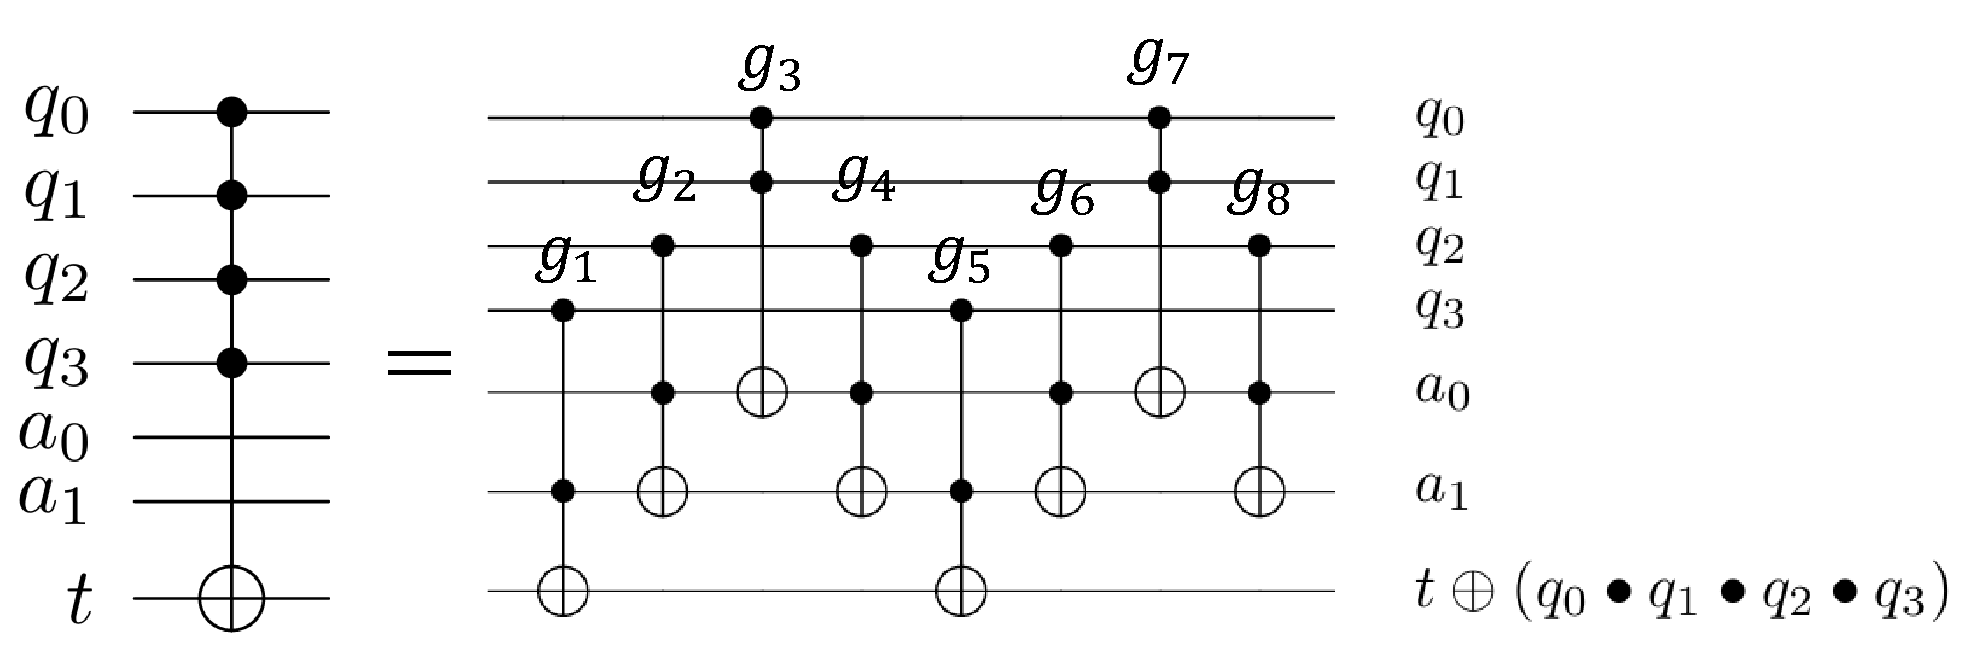
\includegraphics[width=0.95\linewidth]{img/barenco.pdf}
\caption{Example of decomposition of MCT gate into Toffoli gates}
\label{barenco}
\end{figure}
In Figure~\ref{barenco}, the MCT gate is decomposed into Toffoli gates using auxiliary bits $a_{0} and a_{1}$ with undefined values.
If the number of control bits of the MCT gate is $c$, the MCT gate can be decomposed into $4(c-2)$ Toffoli gates using $c-2$ auxiliary bits with undefined values\cite{barenco1995elementary}.
In the example in Figure~\ref{barenco}, the MCT gate with 4 control bits is decomposed into 8 Toffoli gates using 2 auxiliary bits with undefined values.

\section{Decomposition method of MCT gates}
In this chapter, we explain the existing \bout{decomposition method\cite{abdessaied2016technology,baker2019decomposing,niemann2019t}} of MCT gates.

Hereafter, the number of control bits of MCT gates is $c$.

\subsection{Method~1}
In this section, we explain the decomposition method \cite{abdessaied2016technology} of MCT gates that uses $c-2$ auxiliary bits with indefinite values. Hereafter, this method will be called Method~1.

\bout{Method~1} is a method to reduce the T-depth of the method \cite{barenco1995elementary} that decomposes MCT gates into Toffoli gates.

In Method~1, the T-depth is reduced by replacing Toffoli gates with out-of-phase $CCiZ, CCi\omega Z$ gates.

\begin{figure}[tbp]
\centering
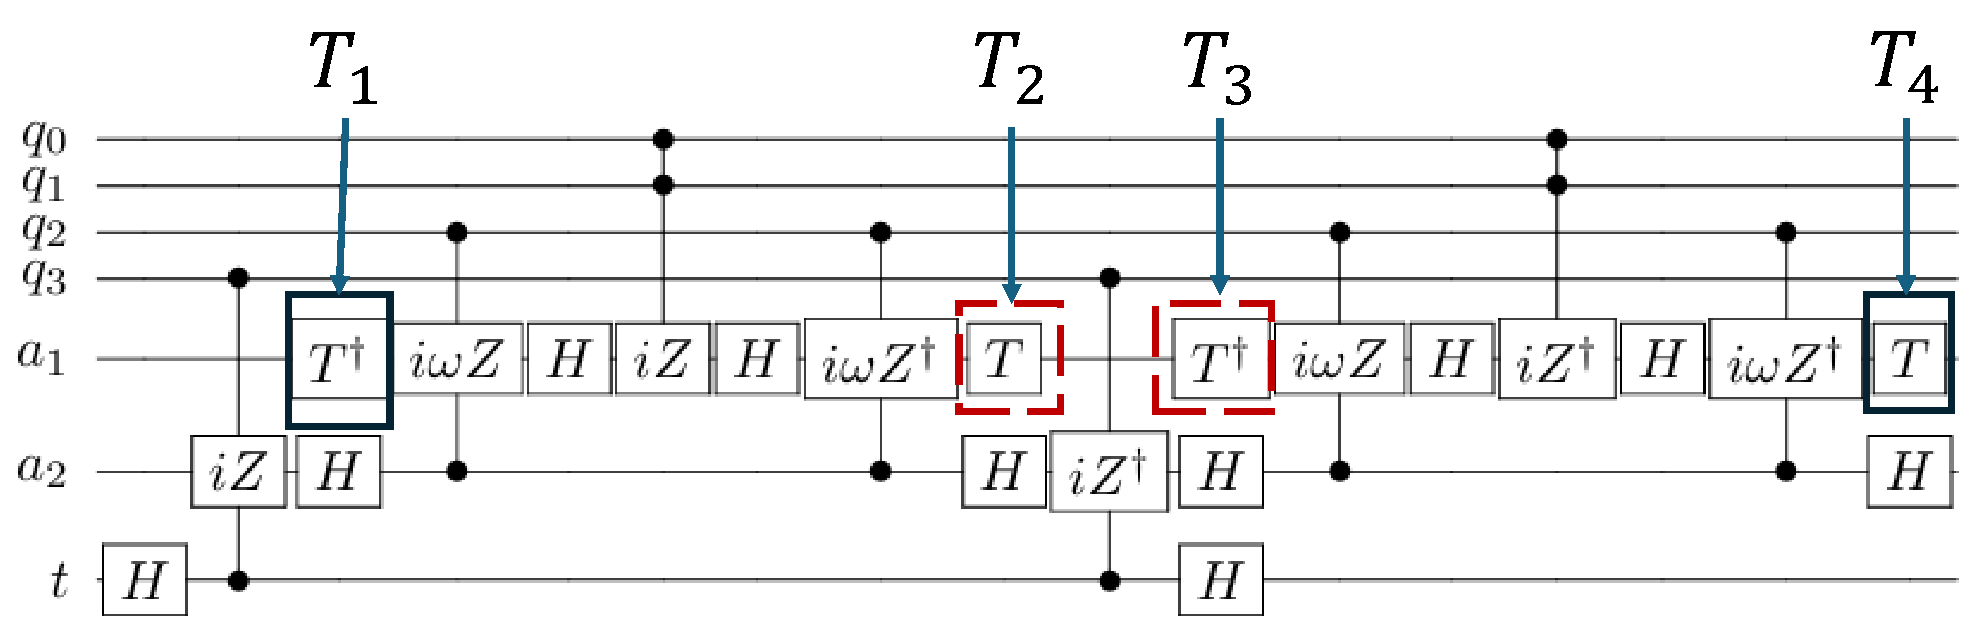
\includegraphics[width=0.95\linewidth]{img/barenco_iz_to_iomegaz.pdf}
\caption{Replacement of $CCiZ$ and $CCiZ^{\dag}$ gates in Figure~\ref{ccz_to_iz_cs} with $CCi\omega Z, T^{\dag}$ gates, respectively.}

\label{barenco_iz_to_iomegaz}

\end{figure}

\begin{figure}[tbp]

\centering

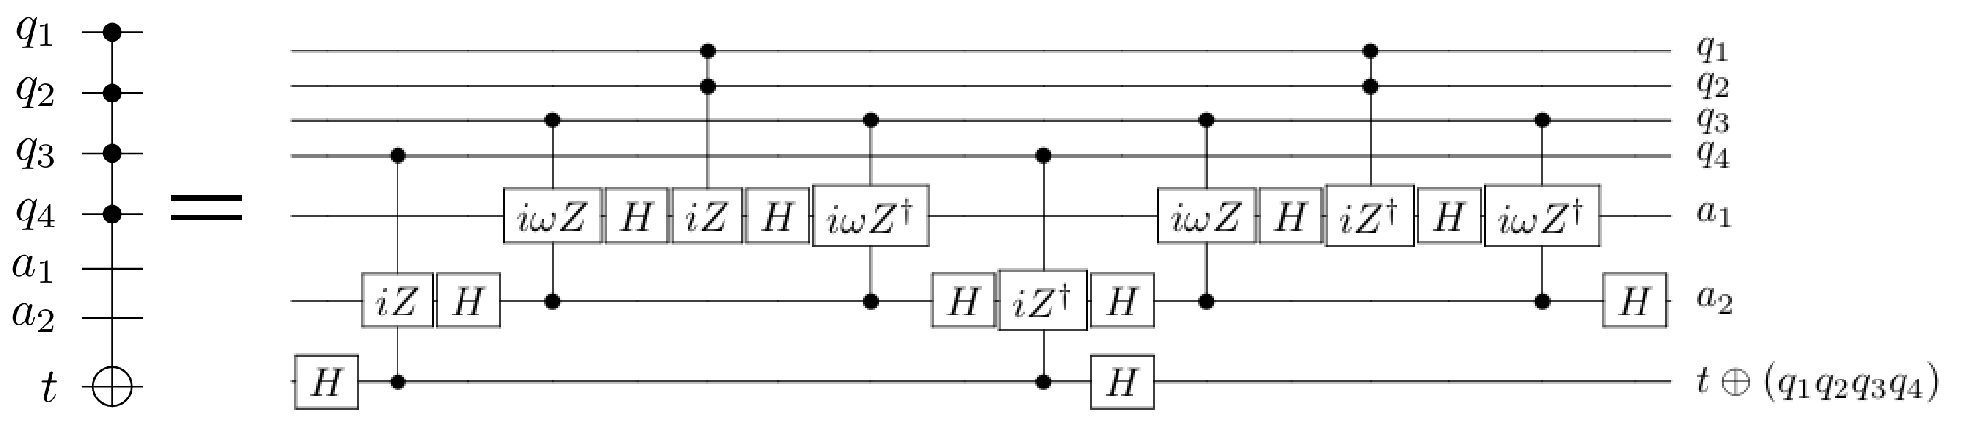
\includegraphics[width=0.9\columnwidth]{img/techmap.pdf}

\caption{Application of method 1 to MCT gates with $c=4$}

\label{techmap}

\end{figure}

\par
Method 1 uses $c-2$ auxiliary bits to decompose the MCT gate into 4 $CCiZ$ gates and $4(c-3)$ $CCi\omega Z$ gates.

The decomposition of the $CCiZ$ gate and the $CCi\omega Z$ gate into Clifford+T is shown in Figure 1 and Figure 2, respectively.

The T-depth of the $CCiZ$ gate is 2, and the T-depth of the $CCi\omega Z$ gate is 1.

Therefore, the maximum T-depth of the MCT gate decomposed by method 1 is $4(c-1)$.

\begin{figure}[tbp]

\centering

\begin{minipage}[b]{0.49\columnwidth}

\centering

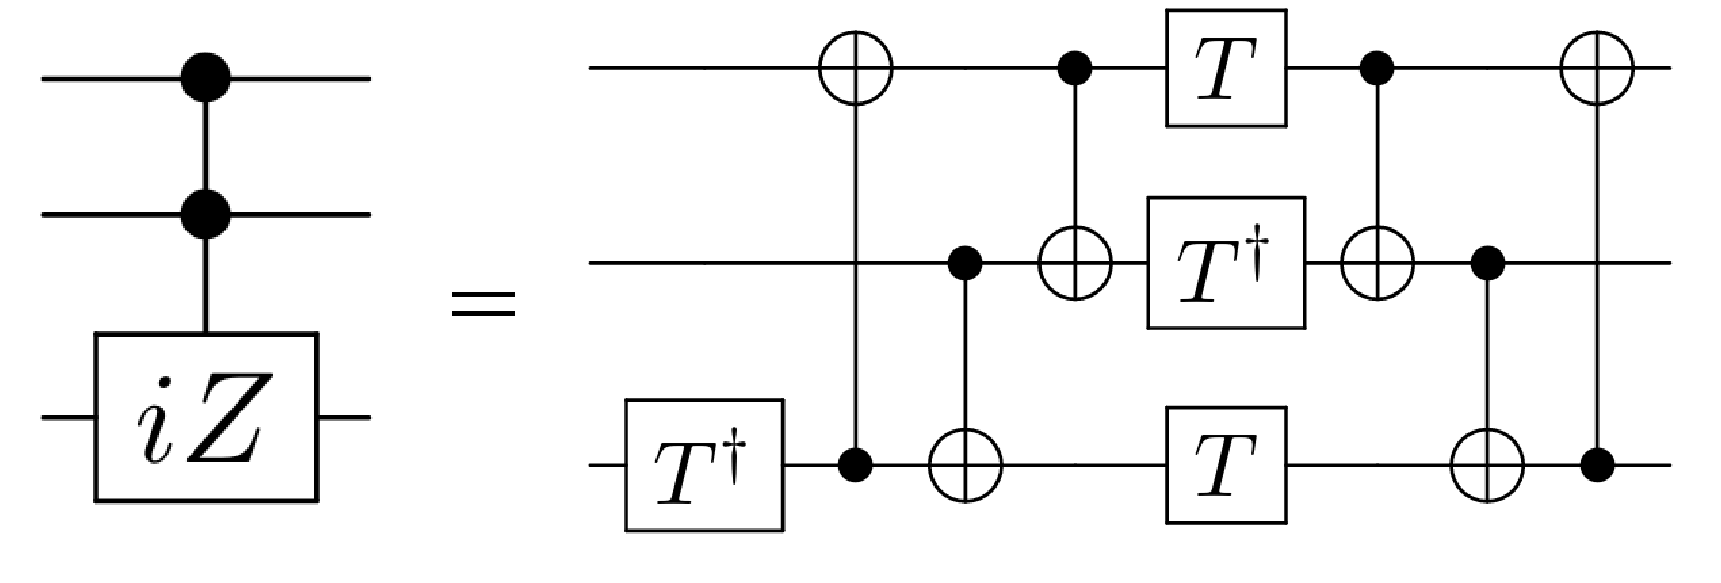
\includegraphics[width=0.9\columnwidth]{img/cciz.pdf}

\caption{Decomposition of $CCiZ$ gate into Clifford+T}

\label{cciz}

\end{minipage}

\begin{minipage}[b]{0.49\columnwidth}

\centering

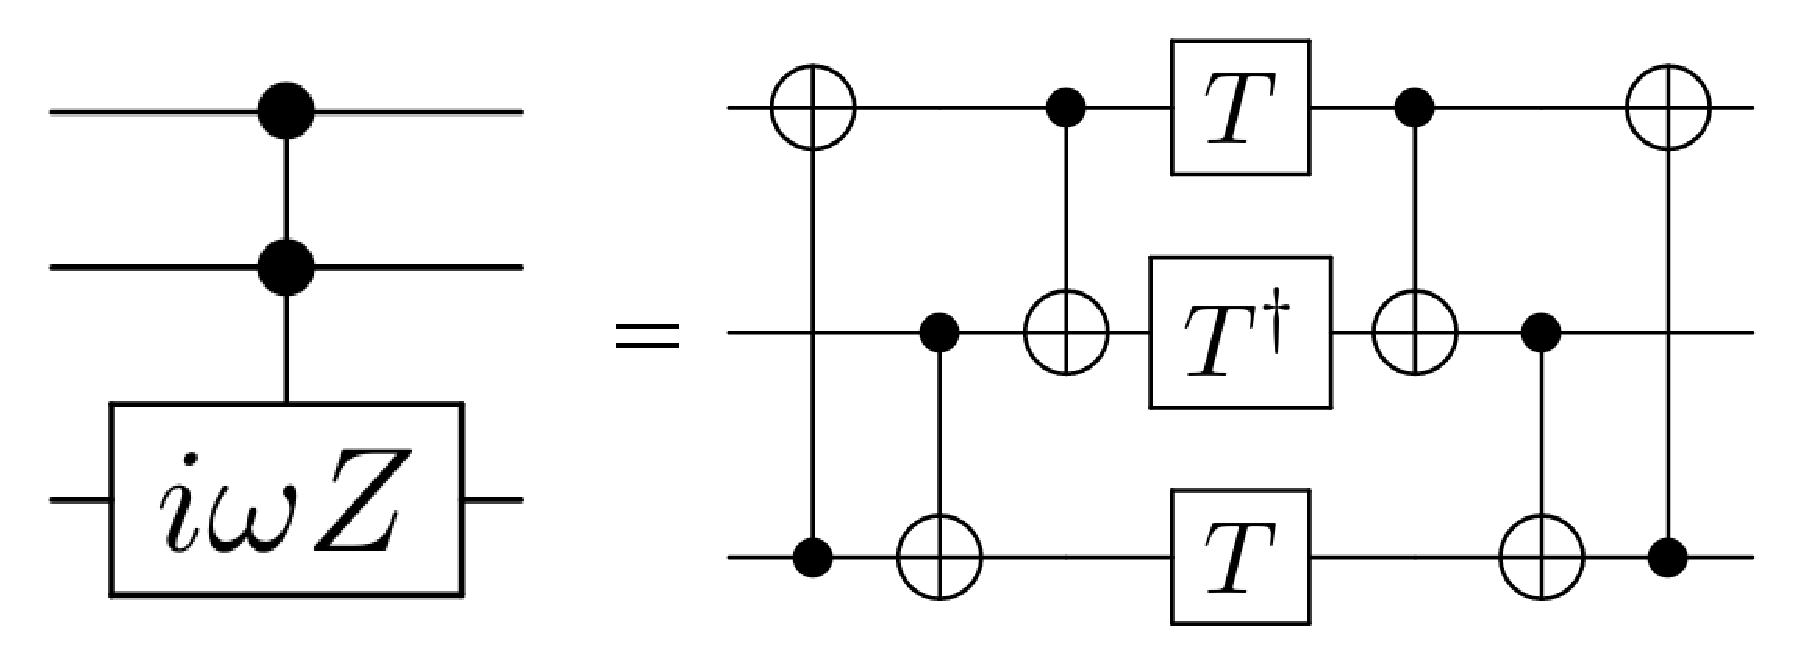
\includegraphics[width=0.9\columnwidth]{img/cciomegaz.pdf}

\caption{$Decomposition of CCi\omega Z$ gate into Clifford+T}
\label{cciomegaz}
\end{minipage}
\end{figure}
\subsection{Method~2}
In this section, we explain the decomposition method \cite{abdessaied2016technology} that uses one auxiliary bit with an undefined value.
Hereafter, we will refer to this method as Method~2.
\par
When there are fewer than $c-2$ auxiliary bits with undefined values, the MCT gate cannot be decomposed using Method~1.
%We explain how to decompose the control bits into two.
\bout{Therefore, we divide the $c$ control bits into two sets of bits.
At this time, we divide them so that the difference in the number of elements in the two sets of bits is within one. }
Then, as shown in Figure~\ref{mimap},
the MCT gate is decomposed into four MCT gates,
$g_{1}, g_{2}, g_{3}, g_{4}$, and four $C\omega S$ gates,
which have the set of split bits as their control bits.
\begin{figure}[tbp]
\centering
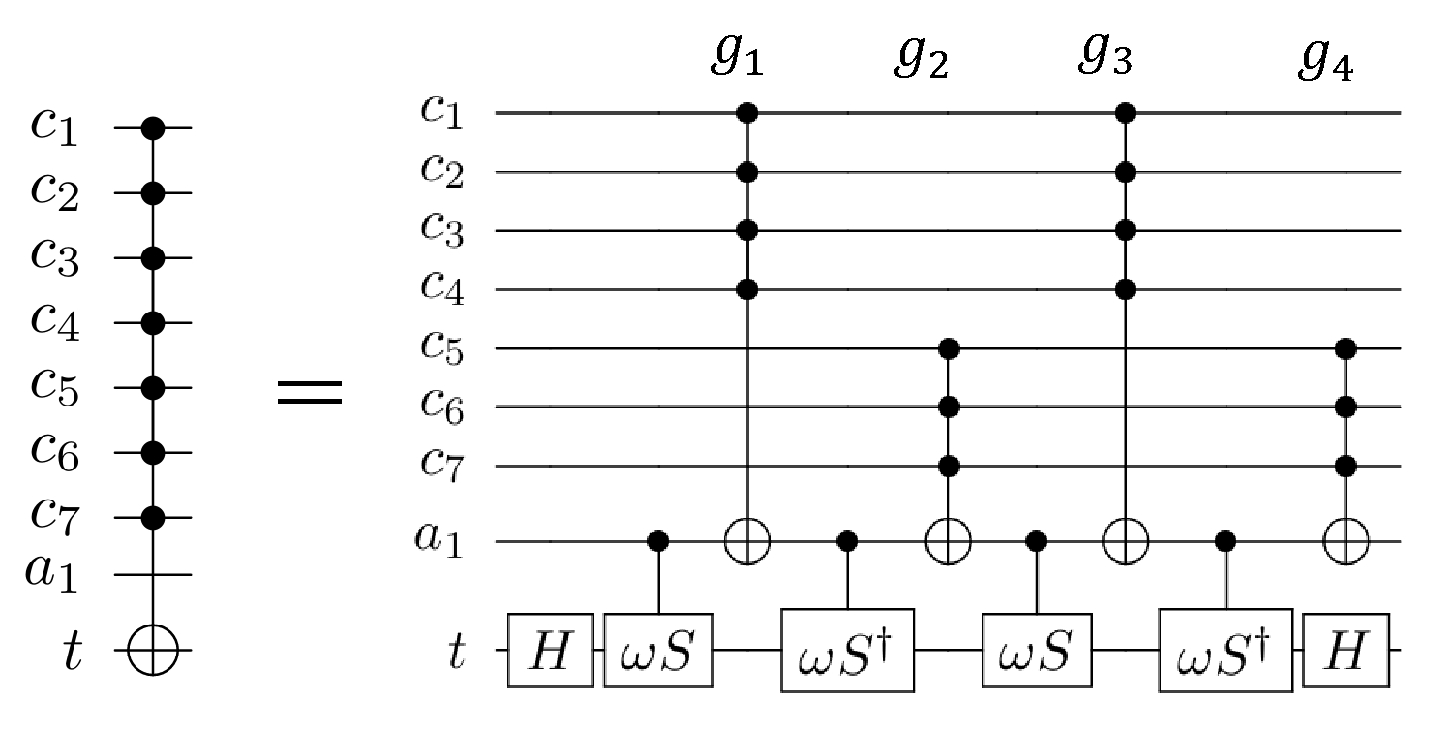
\includegraphics[width=0.95\linewidth]{img/mimapping.pdf}
\caption{Application of method~2 to MCT gate with $c=7$}
\label{mimap}
\end{figure}
Here, $g_{3}$ is a copy of $g_{1}$, and $g_{4}$ is a copy of $g_{2}$.
\begin{figure}[tbp]
\centering
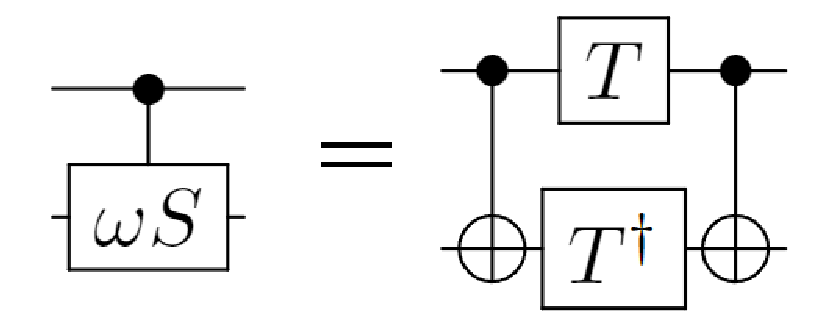
\includegraphics[width=5cm]{img/comegas.pdf}
\caption{Decomposition of $C\omega S$ gate into Clifford+T}
\label{comegas}
\end{figure}
As shown in Figure~\ref{comegas},
the $C\omega S$ gate can be decomposed directly into Clifford+T without using auxiliary bits.
In Method~2,
by applying Method~1 to the four decomposed MCT gates,
the MCT gate can be decomposed into Clifford+T.
\par
In Method~2,
the same auxiliary bits are used to replace $g_{3}$ in Figure~\ref{mimap} with the decomposition of $g_{1}$, and $g_{4}$ with the decomposition of $g_{2}$,
and the T-depth is reduced by decomposing in the reverse order.
\mout{
Figure~\ref{mimap_g2_g4}
shows an example of decomposing $g_{2}$ in Figure~\ref{mimap},
replacing $g_{4}$ with gates of the inverse transformation for the decomposition of $g_{2}$, and decomposing in the reverse order.
$G_{2} and G_{4}$ in Figure~\ref{mimap_g2_g4} represent the decomposition of $g_{2} and g_{4}$.
$G_{4}$ is the gates that make up $G_{2}$ replaced with gates of the inverse transformation, and decomposed in the reverse order. }
\begin{figure}[tbp]
\centering
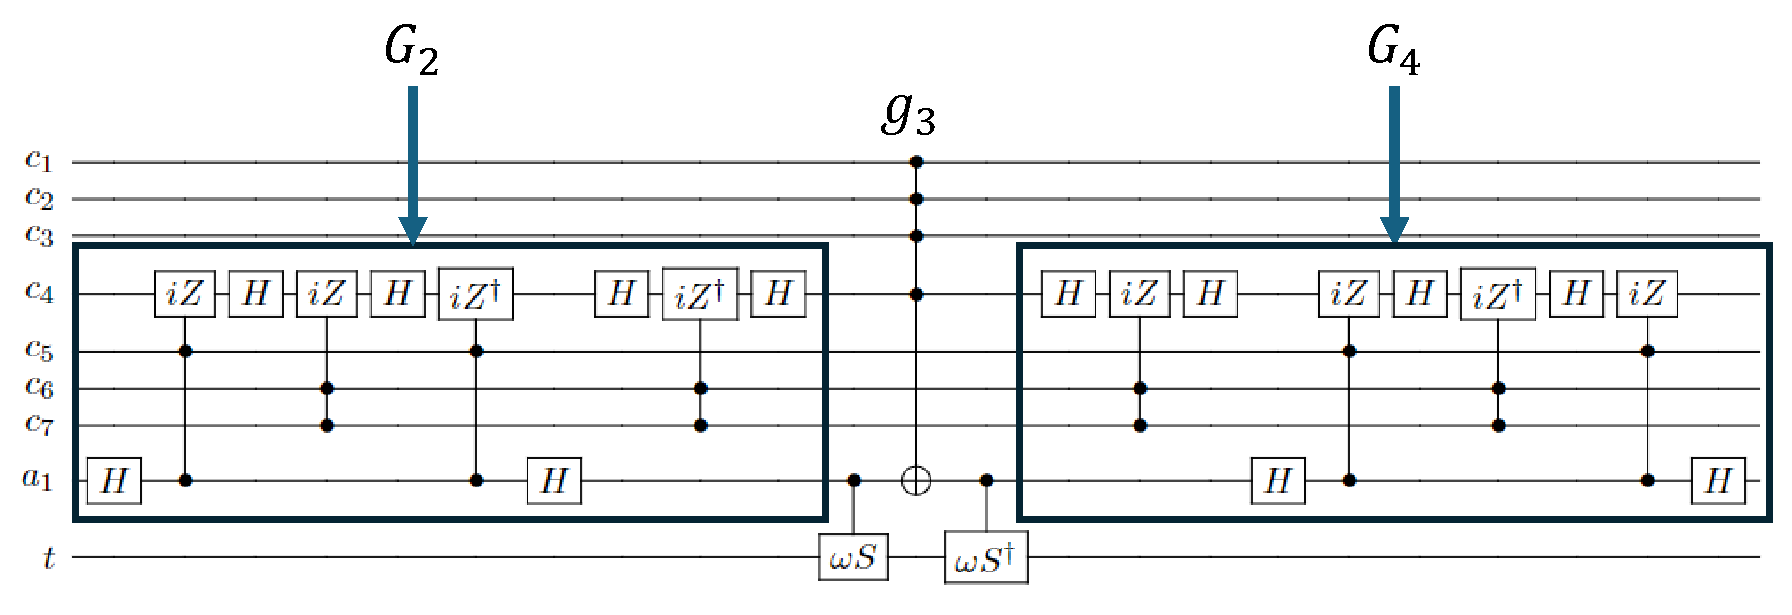
\includegraphics[width=0.95\linewidth]{img/mimap_g2_g4.pdf}
\caption{\mout{An example of decomposing $g_{2}$ in Figure~\ref{mimap}, replacing $g_{4}$ with a gate that is the inverse transformation of the decomposition of $g_{2}$, and decomposing in the reverse order}}
\label{mimap_g2_g4}
\end{figure}
As shown in Figure~\ref{iz_to_iomegaz},
\bout{The $CCiZ gate$ and $CCiZ^{\dag}$ gate can be replaced by the $CCi\omega Z, T^{\dag}$ gate and the $CCi\omega Z^{\dag}, T$ gate, respectively. }
Figure~\ref{mimap_g2_g4_trans} shows an example in which the \bout{$CCiZ gate$ and $CCiZ^{\dag}$ gate in Figure~\ref{mimap_g2_g4} are replaced with the $CCi\omega Z, T^{\dag}$ and $CCi\omega Z^{\dag}, T$ gates, respectively}

.
\mout{
The $T$ gate $T_{4}$ in Figure~\ref{mimap_g2_g4_trans} restores the operation of the $T^{\dag}$ gate $T_{1}$.

These gates can be deleted because their absence does not affect the results of the calculation.

Similarly, $T_{2} and T_{3}$ in Figure~\ref{mimap_g2_g4_trans} can also be deleted.}
\par
In this way, by decomposing the pair $g_{1}, g_{3}$ and the pair $g_{2}, g_{4}$,
a total of eight $CCiZ, CCiZ^{\dag}$ gates can be replaced with $CCi\omega Z, CCi\omega Z^{\dag}$ gates, and the T-depth can be reduced by 8 from before the substitution.

To allow one difference in the control bits and divide evenly,
the total T-depth of the four MCT gates before the substitution when decomposed using method 1 is
$2 \cdot 4(\lfloor \frac{c}{2} \rfloor -1) +2\cdot 4(\lceil \frac{c}{2} \rceil -1)=8(c-1)$.

In addition, because four $C\omega S$ gates are used, the total T-depth of these gates is $4$. 
Therefore, when an MCT gate with $c$ control bits is decomposed using method 2, the maximum T-depth is $8(c-1)-8+4=8c-20$.
\begin{figure}[tbp]
\centering
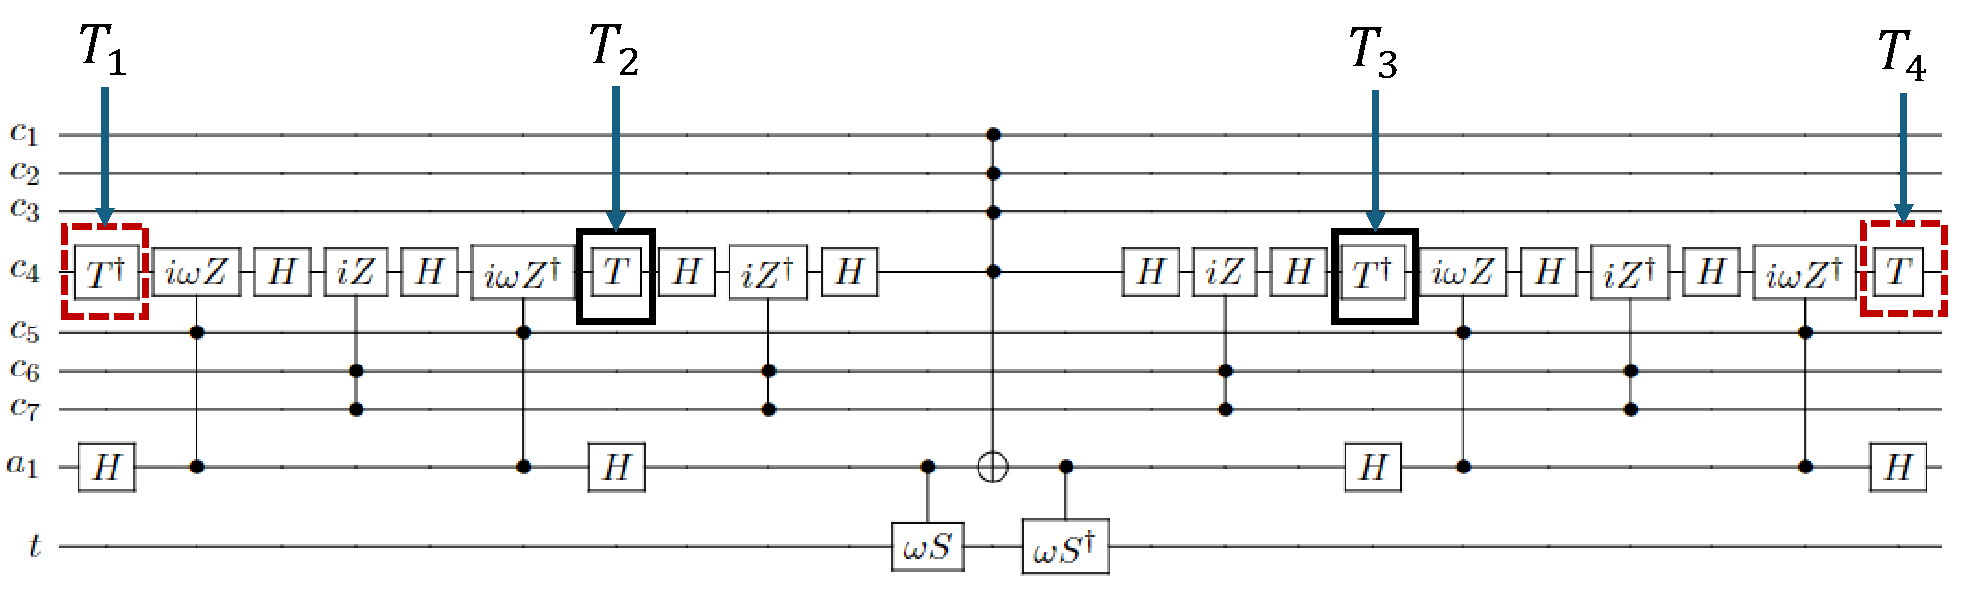
\includegraphics[width=0.95\linewidth]{img/mimap_g2_g4_transform.pdf}
\caption{Figure~\ref{mimap_g2_g4}\bout{An example of replacing the $CCiZ and CCiZ^{\dag}$ gates with $CCi\omega Z, T^{\dag}$ gates and $CCi\omega Z^{\dag}, T$ gates, respectively}}
\label{mimap_g2_g4_trans}
\end{figure}
\subsection{Method~3}
In this section, we explain the method\cite{baker2019decomposing}, which uses 2 to $c-3$ auxiliary bits with indefinite values to decompose MCT gates.
Hereafter, we will refer to this method as Method~3.
As shown in Figure~\ref{baker},

Method~3 is a method to reduce T-depth by decomposing MCT gates $g_{1}$ or $g_{4}$, which require a small number of copies, using many control bits.

In Figure~\ref{baker}, $g_{1}$ has only $g_{7}$ copies,

but $g_{2}$ has $g_{6}, g_{8}, and g_{13}$ copies,

so $g_{1}$ can be said to be a gate with a small number of copies.

For $g_{4}$, the only copy is $g_{10}$.

\par
The decomposition method of Method~3 is explained below.

Let $C$ be a set of $c$ control bits of the MCT gate to be decomposed.

Let $t$ be the target bit of the MCT gate to be decomposed.
\mout{Let $a_{1}, a_{2}, \dots, a_{m}$ be the $m$ auxiliary bits with indefinite values that can be used to decompose MCT gates. }
As shown in Figure~\ref{baker}, once the arrangement of $g_{1}, g_{2}, g_{3}, and g_{4}$ is determined,
the gates to the right of $g_{4}$ are copies of $g_{1}, g_{2}, g_{3}, and g_{4}$, so the decomposition of method~3 can be\rout{determined}.
In other words, once the arrangement of the bits that make up the $m+1$ gates from the left is determined, the decomposition of method~3 can be\rout{determined}.
Let the $m+1$ MCT gates from the left be $g_{1}, \dots, and g_{m+1}$, respectively.
The sets of control bits owned by $g_{1},\dots ,g_{m+1}$ are denoted by $C_{1}, C_{2},\dots ,C_{m+1}$, respectively.

The number of elements in the set is denoted by $|C_{i}|$.

The bits that make up the control bit set $C_{1},\dots ,C_{m+1}$ are determined according to the following procedure.

\begin{enumerate}[Step 1]

\item Move $a_{1},\dots,a_{m}$ one by one to $C_{1},\dots ,C_{m}$.

\item Move elements from $C$ to $C_{i}$ so that the number of elements in $C_{1},\dots,C_{m+1}$ is all 2. 
\item \mout{Move elements from $C$ to $C_{1}$ as long as $C_{1}$ is $|C_{1}|-2 \leq c+m-|C_{1}|$. }
\item \mout{Move the remaining elements of $C$ to $C_{m+1}$ if $|C|=0$ is not true. }
\end{enumerate}
\par
Next, we explain how to determine the target bits of $g_{1},\dots ,g_{m+1}$.
The target bit of $g_{1}$ is the target bit $t$ of the MCT gate before decomposition.
The target bit of $g_{i\geq 2}$ is the bit included in $C_{i-1}$\mout{ distributed in step 1. }
In this way, the bit arrangement of $g_{1},\dots, g_{m+1}$ is determined.
\par
Once the bits that make up $g_{1},\dots,g_{m+1}$ have been determined,
the gates are placed in the order of equation~\ref{eq:bakerhaiti} from the left side of the circuit.
\begin{equation}\label{eq:bakerhaiti}
\{g_{1}, g_{2}, \dots, g_{m+1}\},\{g_{m},g_{m-1}, \dots, g_{1}\}, \{g_{2}, g_{3} \dots, g_{m+1}\}, \{g_{m}, g_{m-1}, \dots, g_{2}\}
\end{equation}
Among the gates placed, gates with three or more control bits are decomposed using method 1.
\begin{figure}[tbp]
\centering
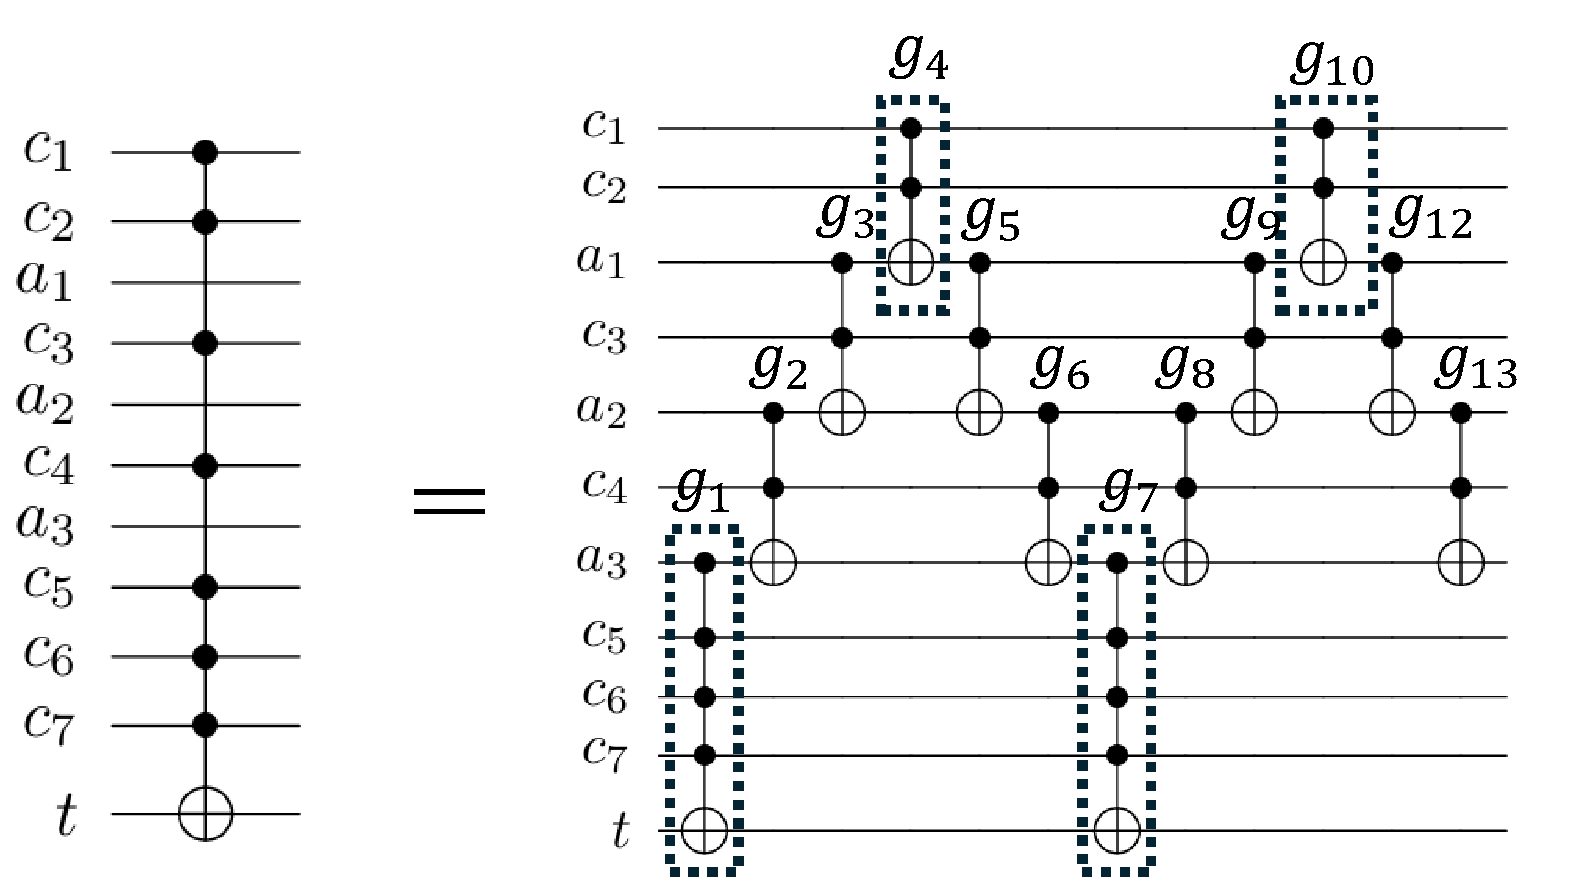
\includegraphics[width=0.95\linewidth]{img/baker.pdf}
\caption{Example of application of method ~3 to MCT gate with $c=7$ and 3 undefined auxiliary bits}
\label{baker}
\end{figure}
\par
The Toffoli gate that appears when applying the decomposition of method ~3 to the MCT gate can be replaced with a $CCiZ, CCi\omega Z$ gate.
We will explain this method.
First, the Toffoli gate in Figure ~\ref{baker} can be replaced with a $CCiZ, CCiZ^{\dag}$ gate.
An example is shown in Figure ~\ref{baker_cciz}.
\begin{figure}[tbp]
\centering
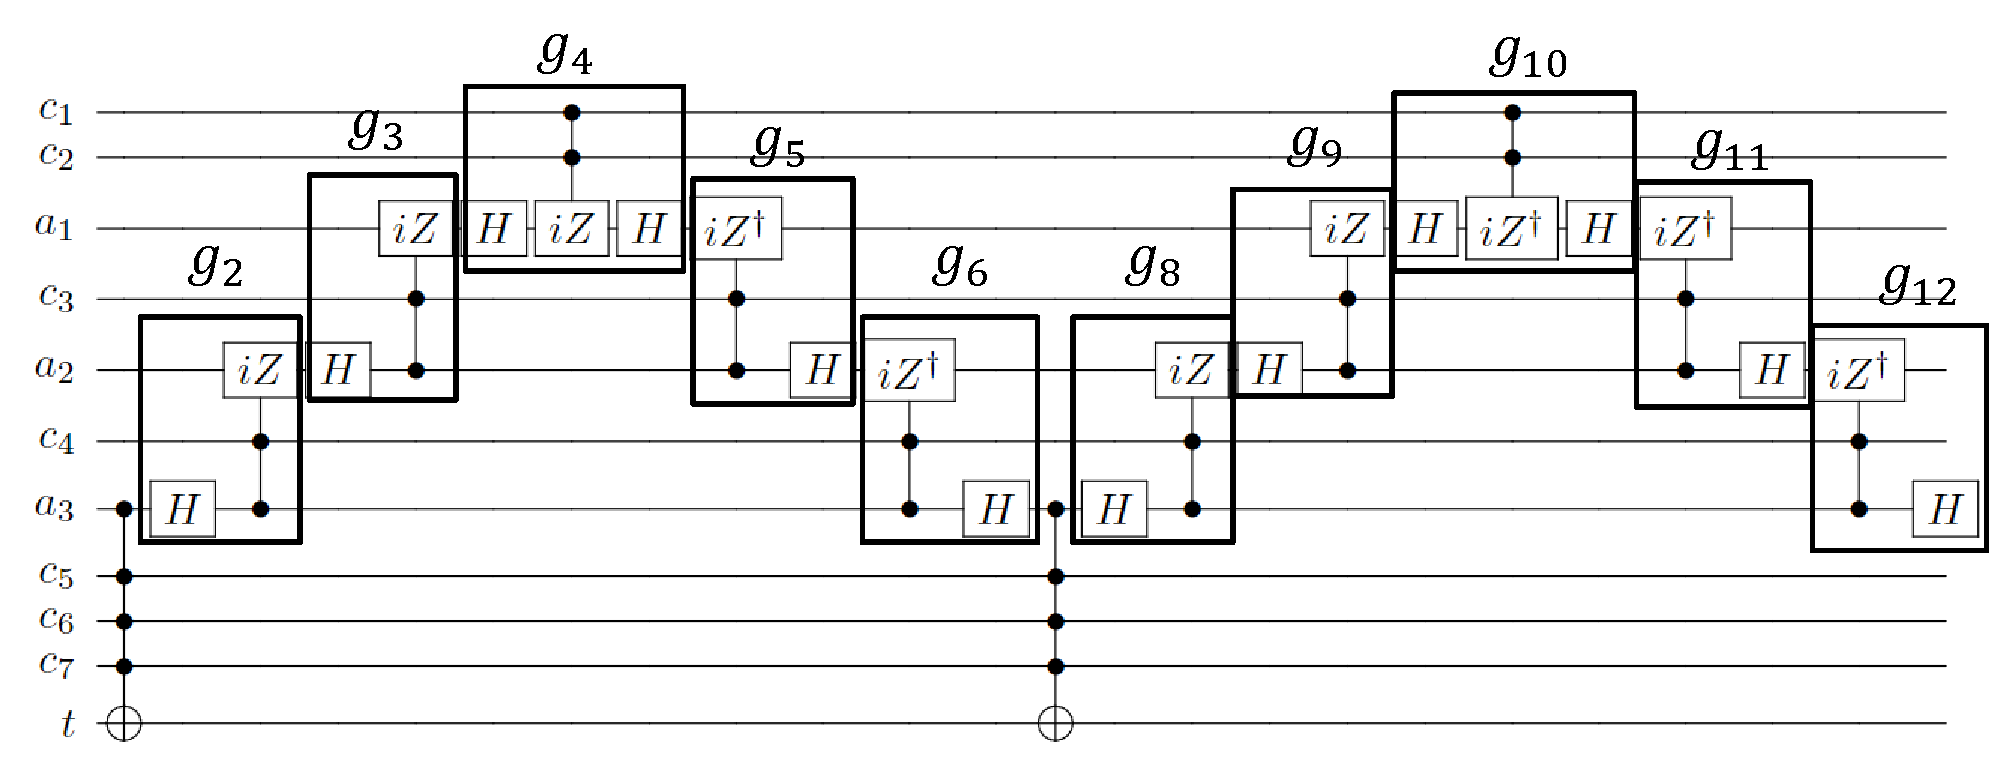
\includegraphics[width=0.95\linewidth]{img/baker_izgate_transform.pdf}
\caption{Replacement of the Toffoli gate in Figure~\ref{baker} with a $CCiZ$ gate}
\label{baker_cciz}
\end{figure}
A pair of Toffoli gates with the same input and output bits is
Figure~\ref{toffoli_transform} $CCZ$ gates can be replaced with $CCiZ$ gates as shown in Figure~\ref{zgate_transform}.

As shown in Figure~\ref{zgate_to_iz},

$CCZ$ gates can be considered to be the same as the target bit and the control bit.

As shown in Figure~\ref{zgate_to_iz}, $CCZ$ gates can be replaced with $CCiZ$ gates and $CS$ gates, or $CCiZ^{\dag}$ gates and $CS^{\dag}$ gates.

The $CS$ gates and $CS^{\dag}$ gates arranged as shown in Figure~\ref{izgate_transform} cancel each other's operations.

Therefore, the same operation can be expressed even if the $CS$ gates and $CS^{\dag}$ gates are eliminated.

In this way, a pair of Toffoli gates with the same input and output can be replaced with a pair of $CCiZ, CCiZ^{\dag}$ gates.
Therefore, the Toffoli gate in Figure~\ref{baker} can be replaced with $CCiZ, CCiZ^{\dag}$ gates as shown in Figure~\ref{baker_cciz}.
\par
As shown in Figure~\ref{baker_cciomegaz},

\bout{$CCiZ, CCiZ^{\dag}$ gates in Figure~\ref{baker_cciz} can be replaced with $CCi\omega Z$ gates and $T^{\dag}$ gates,

$CCi\omega Z^{\dag}$ gates and $T$ gates, respectively. }

$T, T^{\dag}$ gates in Figure~\ref{baker_cciomegaz} can be deleted because their operations cancel each other out.
In addition, for the $T^{\dag}, T$ gates $T_{1}, T_{8}$ and $T_{2}, T_{7}$ in Figure~\ref{baker_cciomegaz}, the operation of the \bout{$T^{\dag}$} gates of $T_{1}, T_{2}$ on the left side is restored by the \bout{$T$ gates} of $T_{7}, T_{8}$ on the right side. 
These gates can also be deleted because their absence does not affect the results of the operation.
In this way, the Toffoli gates that appear in the decomposition of Method~3 can be replaced with $CCiZ, CCi\omega Z$ gates.
\begin{figure}[tbp]
\centering
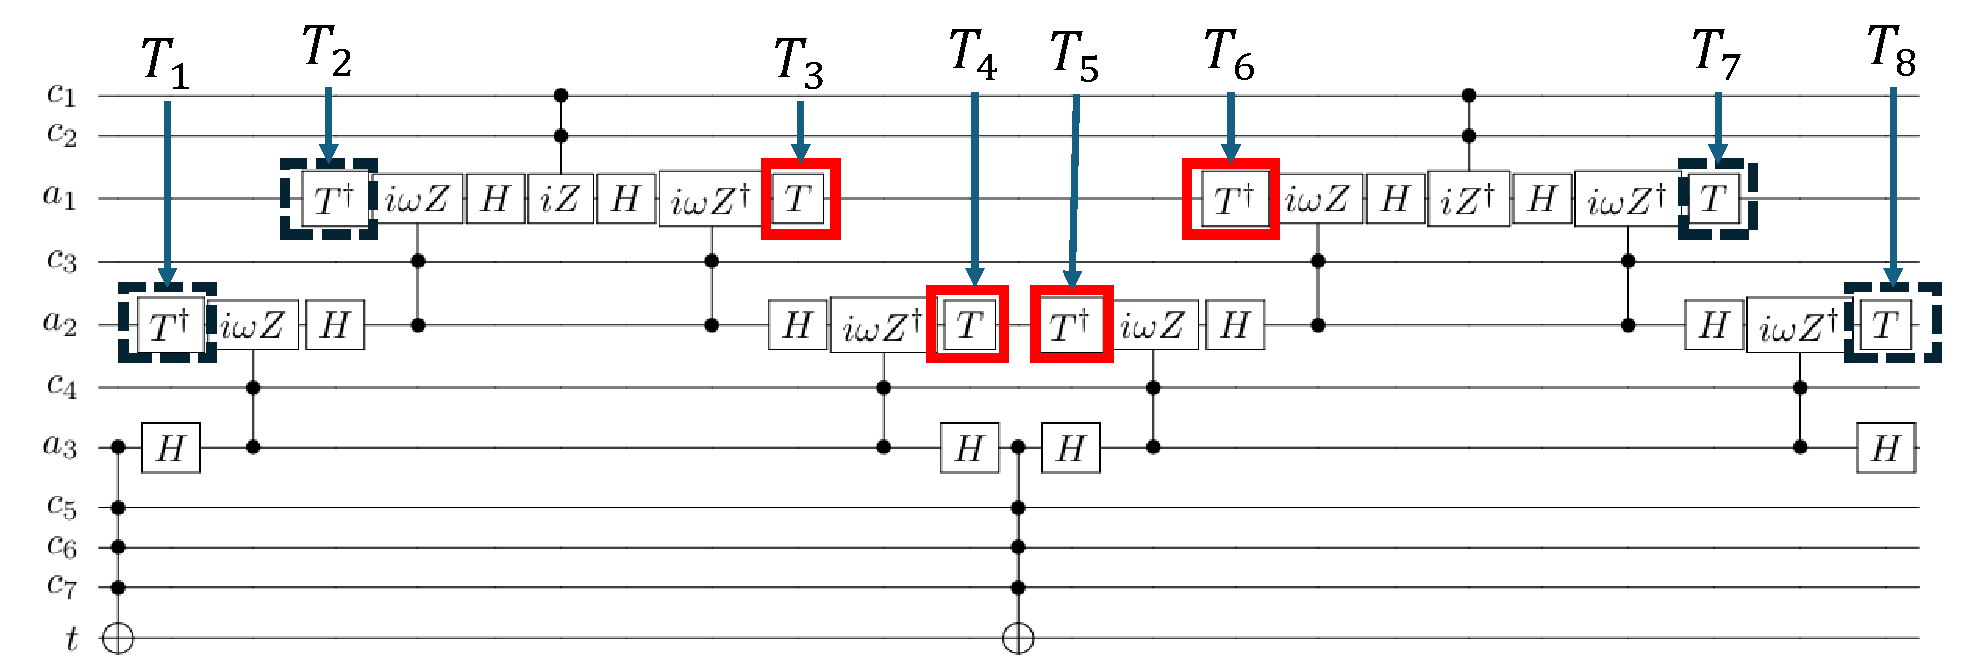
\includegraphics[width=0.95\linewidth]{img/baker_iomegaz.pdf}
\caption{An example in which the \bout{$CCiZ, CCiZ^{\dag}$ gates in Figure~\ref{baker_cciz} are replaced with $CCi\omega Z, T^{\dag}$ gates and $CCi\omega Z^{\dag}, T$ gates, respectively}}
\label{baker_cciomegaz}
\end{figure}
\subsection{Method~4}
In this section,
we explain the decomposition method\cite{niemann2019t} of MCT gates using auxiliary bits whose value is 0.
From now on, this method will be called Method~4.
Method~4 decomposes MCT gates by dividing the cases into based on the number of auxiliary bits whose value is 0, $k$, used in the decomposition.
Also, let $d$ be the number of auxiliary bits with indefinite values used in the decomposition.

Let $a_{1},\dots, a_{k}$ be the $k$ auxiliary bits with a value of 0. Let $c$ be the number of control bits of the MCT gate to be decomposed.

\subsection*{In the case of $1\leq k \leq \frac{c}{2}$}

In the case of $1\leq k \leq \frac{c}{2}$,
the MCT gate to be decomposed is decomposed into three stages of MCT gates, as shown in Figure~\ref{niemann}.

Method~1 is applied to each of the decomposed MCT gates to perform the decomposition.

In Method~4, as shown in Figure~\ref{niemann},
the T-depth is reduced by arranging MCT gates in parallel in the first and third stages by the number of $k$.

\par
We will explain how to decompose MCT gates into three stages.
First, the $c$ control bits of the MCT gate to be decomposed are divided into a set of $k+1$ control bits $C_{1},\dots,C_{k+1}$.
The number of elements in this divided set of control bits is denoted as $|C_{i}|$.
The arrangement of the three-stage MCT gates is as follows.
\begin{enumerate}[First stage]
\item $C_{1},\dots,C_{k}$ are the respective control bits, and $k$ MCT gates are placed with $a_{1},\dots,a_{k}$ as their respective target bits.
\item $C_{k+1}$ and the $k$ auxiliary bits $a_{1},\dots,a_{k}$ are the control bits, and an MCT gate with the target bit $t$ of the original MCT gate as the target bit is placed in the second stage.
\item The third row contains the same $k$ MCT gates as the first row.

The third row MCT gate restores the value of the ancillary bits that are 0 to 0.

\end{enumerate}
\begin{figure}[tbp]

\centering

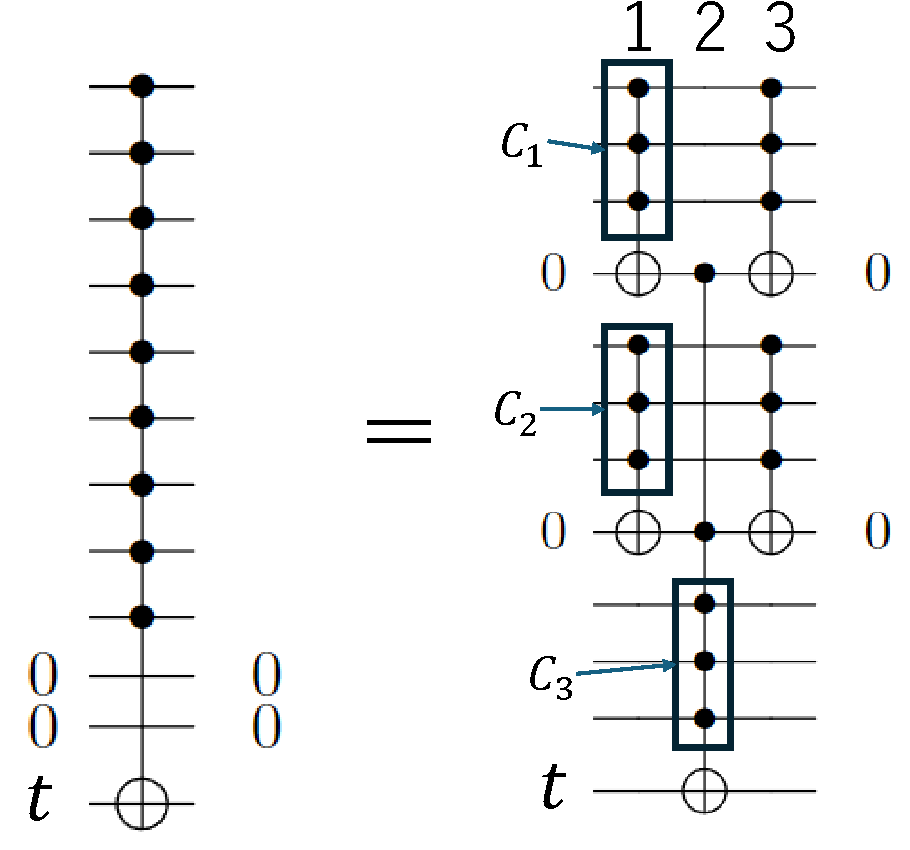
\includegraphics[width=0.95\linewidth]{img/niemann.pdf}

\caption{Decomposition example of MCT gate for $c=9$ using two ancillary bits with a value of 0}

\label{niemann}

\end{figure}

\par
Method~1 is used to decompose the MCT gates arranged in three rows.

Therefore, to decompose these MCT gates,
ancillary bits with undefined values are required according to the number of control bits for each row.

The number of ancillary bits with undefined values required for each row must be considered,

and it is necessary to determine
$C_{1},\dots,C_{k+1}$.

\par
The second row MCT gate has $k+|C_{k+1}|$ control bits.
Therefore, to apply method ~1 to the second-stage MCT gate,
$k+|C_{k+1}-2|$ auxiliary bits with indefinite values are required.
Bits not used in the second-stage MCT gate can be used as auxiliary bits with indefinite values.
Therefore,
$|C_{1}|+,\dots, +|C_{k}|$ bits used as control bits in the first stage
can be used as auxiliary bits with indefinite values in the second-stage MCT gate.
To apply the decomposition of method ~1 to the second-stage MCT gate,
equation ~\ref{eq:2danme} must be satisfied.
\begin{equation}\label{eq:2danme}
d+|C_{1}|+\dots +|C_{k}|\geq (k+|C_{k+1}|)-2
\end{equation}
\par
To apply method~1 to the MCT gates in the first and third stages,
$(|C_{1}|-2)+\dots+(|C_{k}|-2)$ auxiliary bits with undefined values are required.
The bits not used in the first and third stages can be used as undefined auxiliary bits.
Therefore,
$|C_{k+1}|$ bits used as control bits in the second stage and
the target bit $t$ in the second stage can be used as undefined auxiliary bits.
In addition, considering the number $d$ of undefined auxiliary bits used in the decomposition,
equation \ref{eq:13danme} must be satisfied to apply method~1 to the MCT gates in the first and third stages.
\begin{eqnarray}\label{eq:13danme} d+|C_{k+1}|+1&\geq& (|C_{1}|-2)+\dots+(|C_{k}|-2)=|C_{1}|+\dots+|C_{k}|-2k \end{eqnarray} \par $C_{1}+\dots +C_{k+1}=c$ and From the expression~\ref{eq:2danme} and the expression~\ref{eq:13danme}, The formula ~\ref{eq:seiyaku} can be derived.
\begin{equation}\label{eq:seiyaku}
\frac{c+2-k+d}{2}\geq|C_{k+1}|\geq \frac{c-2k-d-1}{2}
\end{equation}
When decomposing MCT gates, if the value of $C_{k+1}$ is set to satisfy equation ~\ref{eq:seiyaku},
method ~1 can be applied to each decomposed MCT gate.
\par
If the MCT gates are simply decomposed to satisfy equation ~\ref{eq:seiyaku},
the overall T-depth may become large.
Therefore,
$C_{1},\dots,C_{k+1}$ must be determined so that the overall \bout{T-depth becomes small}.
The method for determining this consists of the following three steps.
\begin{enumerate}[Step (1)]
\item $|C_{k+1}|$ is the maximum value that satisfies the formula \ref{eq:seiyaku}.
Then, move the remaining $c-|C_{k+1}|$ control bits evenly to $C_{1},\dots,C_{k}$.
At this time, the difference between $|C_{1}|,\dots,|C_{k}|$ is allowed to be up to 1.
\item Move the control bits from $C_{k+1}$ to $C_{1},\dots,C_{k}$ so that the maximum number of $|C_{1}|,\dots,|C_{k}|$ does not increase.
At this time, move so that $|C_{k+1}|$ satisfies the formula \ref{eq:seiyaku}.
\item
If $k\geq 2$ and three or more control bits can be moved from $C_{k+1}$ so that equation \ref{eq:seiyaku} is satisfied,

move the control bits one by one to $C_{1},C_{2}$ and return to step (2).

If not, end.

\end{enumerate}

Based on the above procedure, $C_{1},\dots,C_{k+1}$ are determined and the MCT gates are decomposed into three stages.

\par
When decomposed using $k=\frac{c}{2}$ auxiliary bits with a value of 0,

as shown in Figure~\ref{niemann_frac_c_2},

the number of control bits for all MCT gates in the first and third stages

is 2.

In this case, the first and third stages are the optimal division of the control bits.

Therefore, even if more auxiliary bits with a value of 0 are added,

the control bits in the first and third stages cannot be further divided.
\begin{figure}[tbp]
\centering
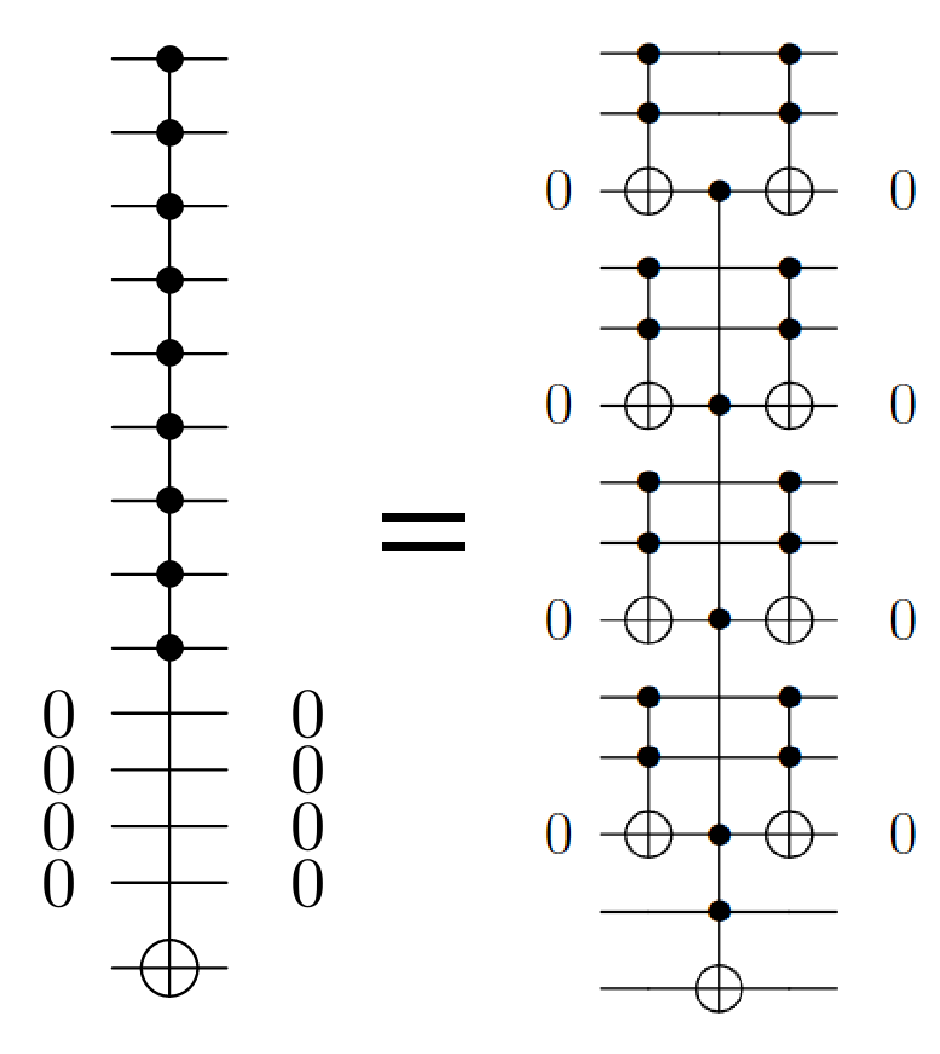
\includegraphics[width=0.95\linewidth]{img/niemann_k_frac_c_2.pdf}
\caption{Example of decomposition of MCT gate $c=9$ using four auxiliary bits with a value of 0}
\label{niemann_frac_c_2}
\end{figure}
\subsection*{When $\frac{c}{2} \bout{<} k \leq c-2$}
When $k>\frac{c}{2}$,
first, use $\lfloor\frac{c}{2}\rfloor$ auxiliary bits with a value of 0 to decompose all MCT gates in the first and third stages so that the number of control bits is 2.
In this case, the number of control bits of the MCT gate in the second stage is $c'=c-\lfloor \frac{c}{2}\rfloor$.
The remaining number of auxiliary bits with a value of 0 is $k'=k-\lfloor \frac{c}{2} \rfloor$.

Using the remaining $k'$ auxiliary bits with a value of 0,
\rout{When $k'\leq \frac{c'}{2}$ and when $k' > \frac{c'}{2}$,
the MCT gate with $c'$ control bits in the second stage is decomposed. }
\par
When $k=c-2$,
as shown in Figure~\ref{niemann_c_2},
the number of control bits for all decomposed MCT gates is 2.

Therefore, even if more than $c-2$ auxiliary bits with a value of 0 are added,
the control bits cannot be further divided. 
\begin{figure}[tbp]
\centering
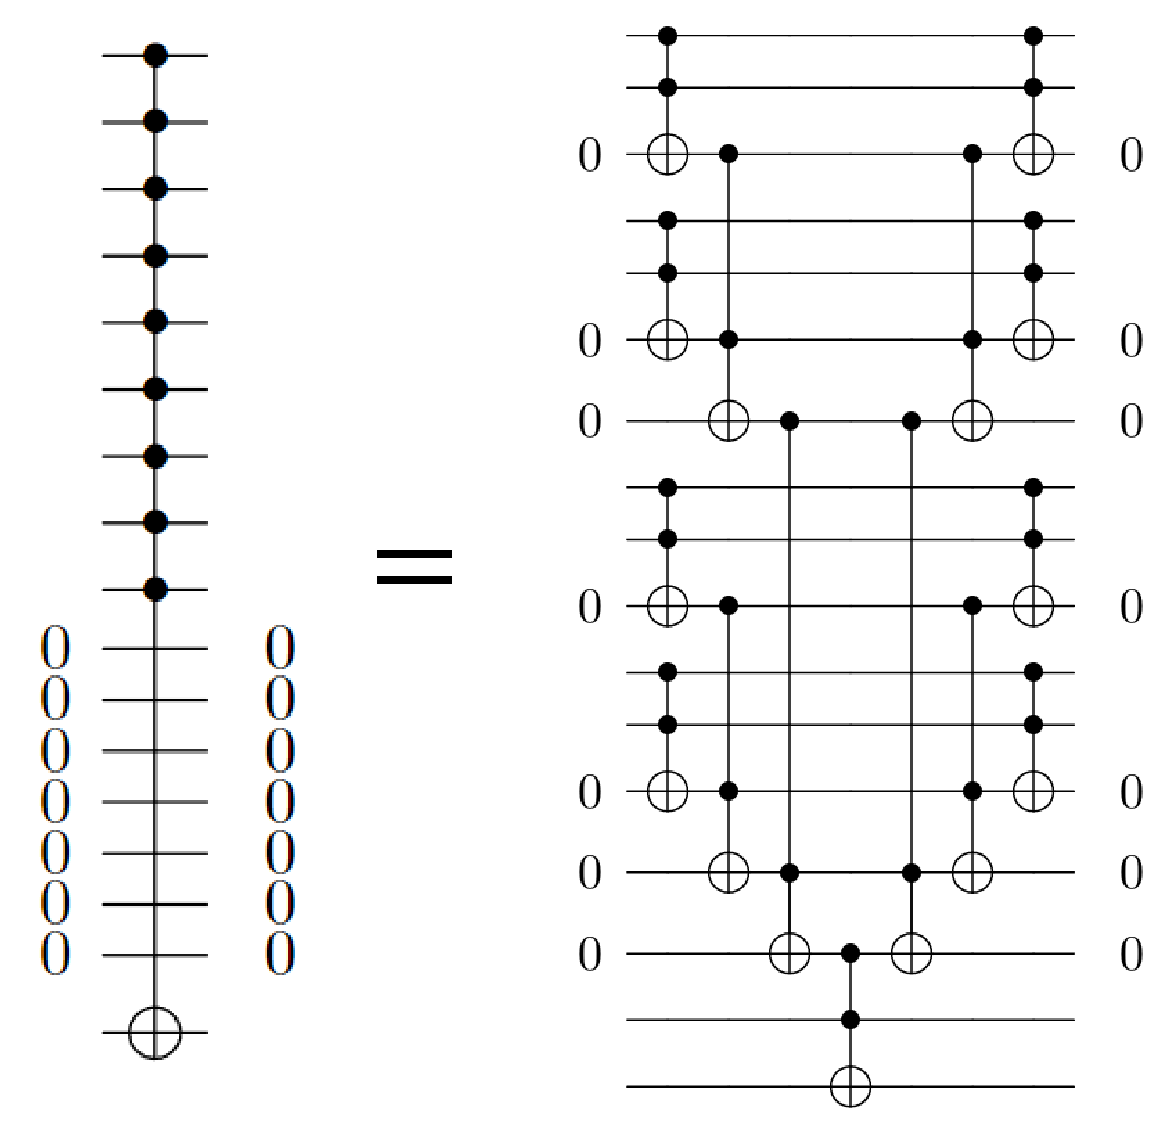
\includegraphics[width=0.95\linewidth]{img/niemann_c_2.pdf}
\caption{Decomposition example of MCT gate for $c=9$ using 7 ancillary bits with value 0}
\label{niemann_c_2}
\end{figure}

%% \input{Mot.tex}
\section{Decomposition method of MCT gate considering T-depth per bit}
In this chapter, we will explain the proposed method of decomposing MCT gate considering T-depth per bit.

\subsection{T-depth per bit}
In this section, we will explain T-depth per bit.

T-depth per bit is calculated for each quantum bit.

\par
We will explain how to calculate T-depth per bit.

Figure~\ref{toffoli_bit}
shows T-depth per bit of decomposition of Toffoli gate.

Let $q_{x}, q_{y}, q_{z}$ be the T-depth per bit of each input quantum bit.

First, the T-depth after execution of the $T$ gate on the left side of Figure~\ref{toffoli_bit}
is the T-depth per bit of that input plus 1.

The CNOT gates enclosed by the black solid lines in Figure~\ref{toffoli_bit}
cannot be executed until the input bits have been executed.
For this reason,
the bitwise T-depth after execution of the CNOT gates enclosed by the black solid lines can be considered to be the maximum bitwise T-depth of the input bits,
i.e., $\max\{q_{x}+1, q_{y}+1\}$.
If we consider the CNOT gates enclosed by the red dotted lines in the same way,
the bitwise T-depth after execution is $\max\{q_{x}+1, q_{y}+1, q_{z}+1\}$.
In this way,
if we calculate the bitwise T-depth from the left side of the Toffoli gate,
the bitwise T-depth after execution of the Toffoli gate can be considered to be $\max\{q_{x},q_{y},q_{z}\}+3$.
\begin{figure}
\centering
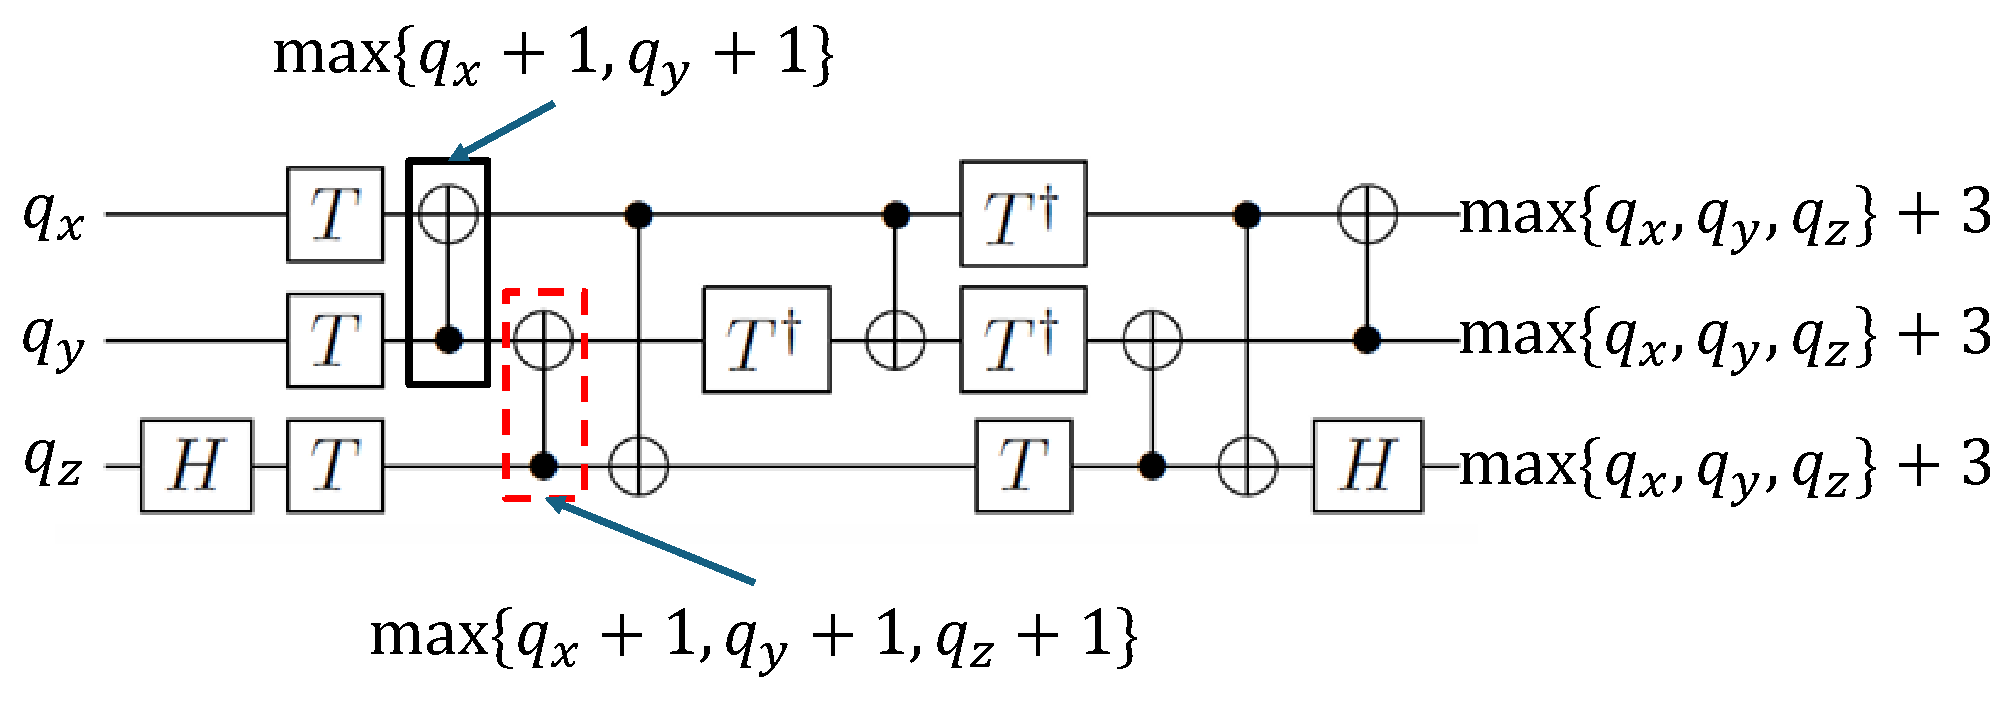
\includegraphics[width=12cm]{img/toffoli_bit.pdf}
\caption{T-depth per bit of Toffoli gate}
\label{toffoli_bit}
\end{figure}
\par
The T-depth per bit can be calculated from gates that can be decomposed into Clifford+T without using auxiliary bits.
Table~\ref{tab:gate_tdepth} shows the T-depth after executing gates that can be decomposed into Clifford+T without using auxiliary bits.
Based on Table~\ref{tab:gate_tdepth},
the T-depth per bit of the circuit can be obtained by calculating the T-depth per bit from the left side of the circuit.
\begin{table}[tbp]
\centering
\caption{T-depth after execution of gates that can be decomposed into Clifforf+T without using auxiliary bits}
\label{tab:gate_tdepth}
\begin{tabular}{c|cc}
Gate name &qubits used &T-depth after execution \\ \hline
$T, T^{\dag}$ &$q_{x} $ &$q_{x}+1$ \\
$H, NOT$ &$q_{x}$ &$q_{x}$ \\
$CNOT$ &$q_{x}, q_{y}$ &$\max\{q_{x}, q_{y}\}$ \\
\bout{Toffoli} &$q_{x}, q_{y}, q_{z}$&$\max\{q_{x},q_{y},q_{z}\}+3$\\ 
$CCiZ, CCiZ^{\dag} $&$q_{x}, q_{y}, q_{z}$&$\max\{q_{x},q_{y},q_{z}\}+2$\\
 $CCi\omega Z, CCi\omega Z^{\dag}$&$q_{x}, q_{y}, q_{z}$&$\max\{q_{x},q_{y},q_{z}\}+1$\\
 $C\omega S, C\omega S^{\dag}$ &$q_{x}, q_{y} $&$\max\{q_{x},q_{y}\}+1 $\\
 \end{tabular} \end{table}
\par
Figure~\ref{bit_tdepth} shows an example of calculating the T-depth for each bit based on Table~\ref{tab:gate_tdepth}.

The T-depth for each input bit in Figure~\ref{bit_tdepth} is all set to 0.

The maximum T-depth for Figure~\ref{bit_tdepth} is 12,
and the minimum T-depth is 8.

Figure~\ref{bit_tdepth} shows the T-depth for each bit obtained by decomposing an MCT gate with 4 control bits using Method~1.

When the T-depth for each bit is calculated in this way, there will be differences in the T-depth for each bit.

For this reason, by prioritizing bits with smaller T-depths

and decomposing the MCT gate, the T-depth for the entire circuit can be reduced.
\begin{figure}
\centering
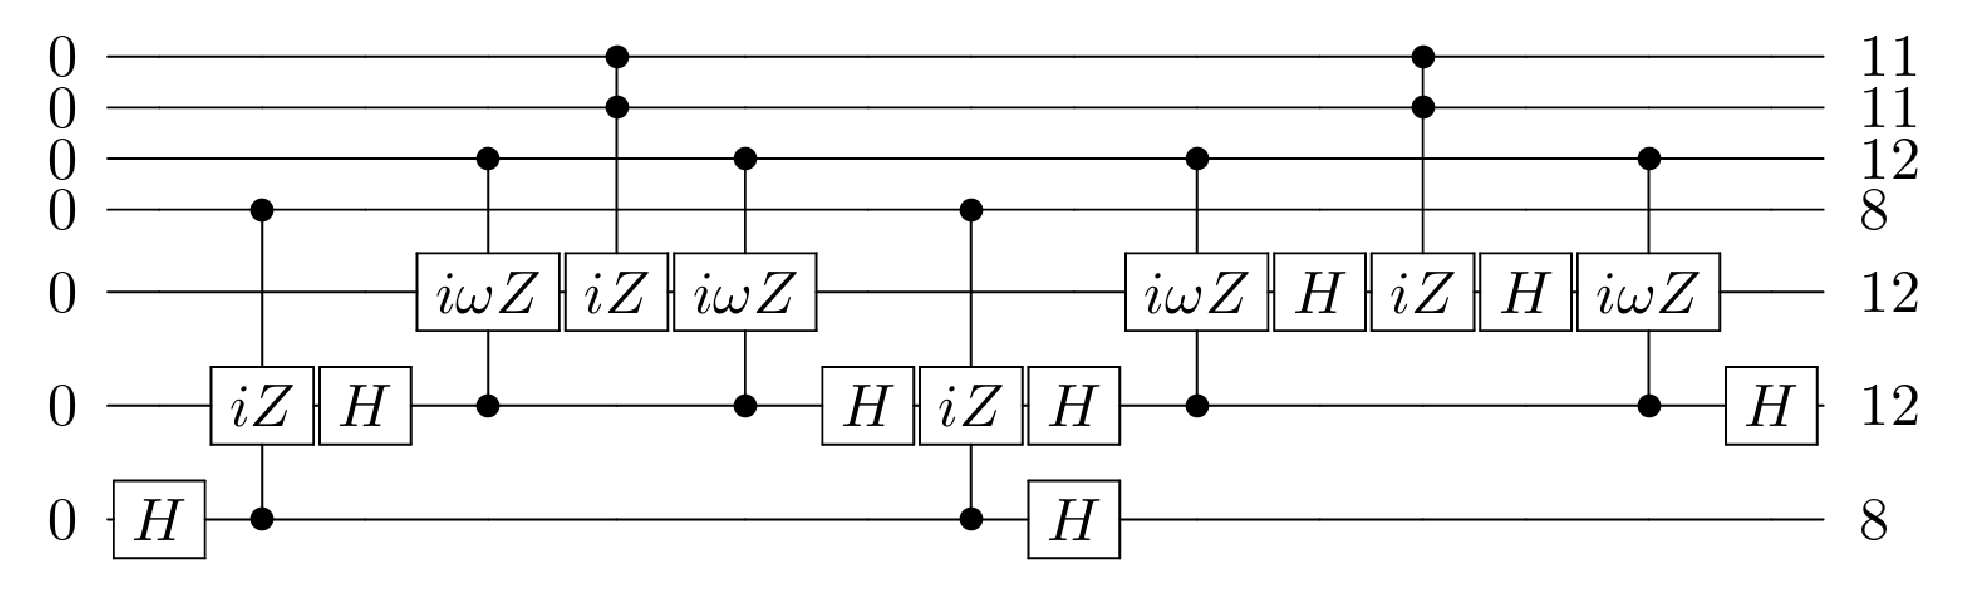
\includegraphics[width=14cm]{img/bit_tdepth.pdf}
\caption{T-depth per bit of the circuit in Figure~\ref{techmap}}
\label{bit_tdepth}
\end{figure}
\par
Figure~\ref{consider_tdepth} shows an example of decomposition of an MCT gate with three control bits, taking into account the T-depth per bit.
In Figure~\ref{consider_tdepth}, there is a difference in the T-depth of each bit on the input side.
Therefore, when applying decomposition that takes into account the T-depth of bits to method~1,
the T-depth can be reduced by using bits with the smallest T-depth in ascending order.
Figure~\ref{bad_consider_tdepth} shows an example in which the maximum T-depth after decomposition deteriorates due to bit selection.
In the example of Figure~\ref{bad_consider_tdepth},
if $q_{4}$ bits are used for the first gate $g_{1}$,
the maximum T-depth after execution of the \bout{subsequent} gates will be 20, since the T-depth depends on that value.
On the other hand, in Figure~\ref{consider_tdepth},
the maximum T-depth of the bits after decomposition is reduced by using the control bits and auxiliary bits in ascending order of T-depth.
\begin{figure}[tbp]
\centering
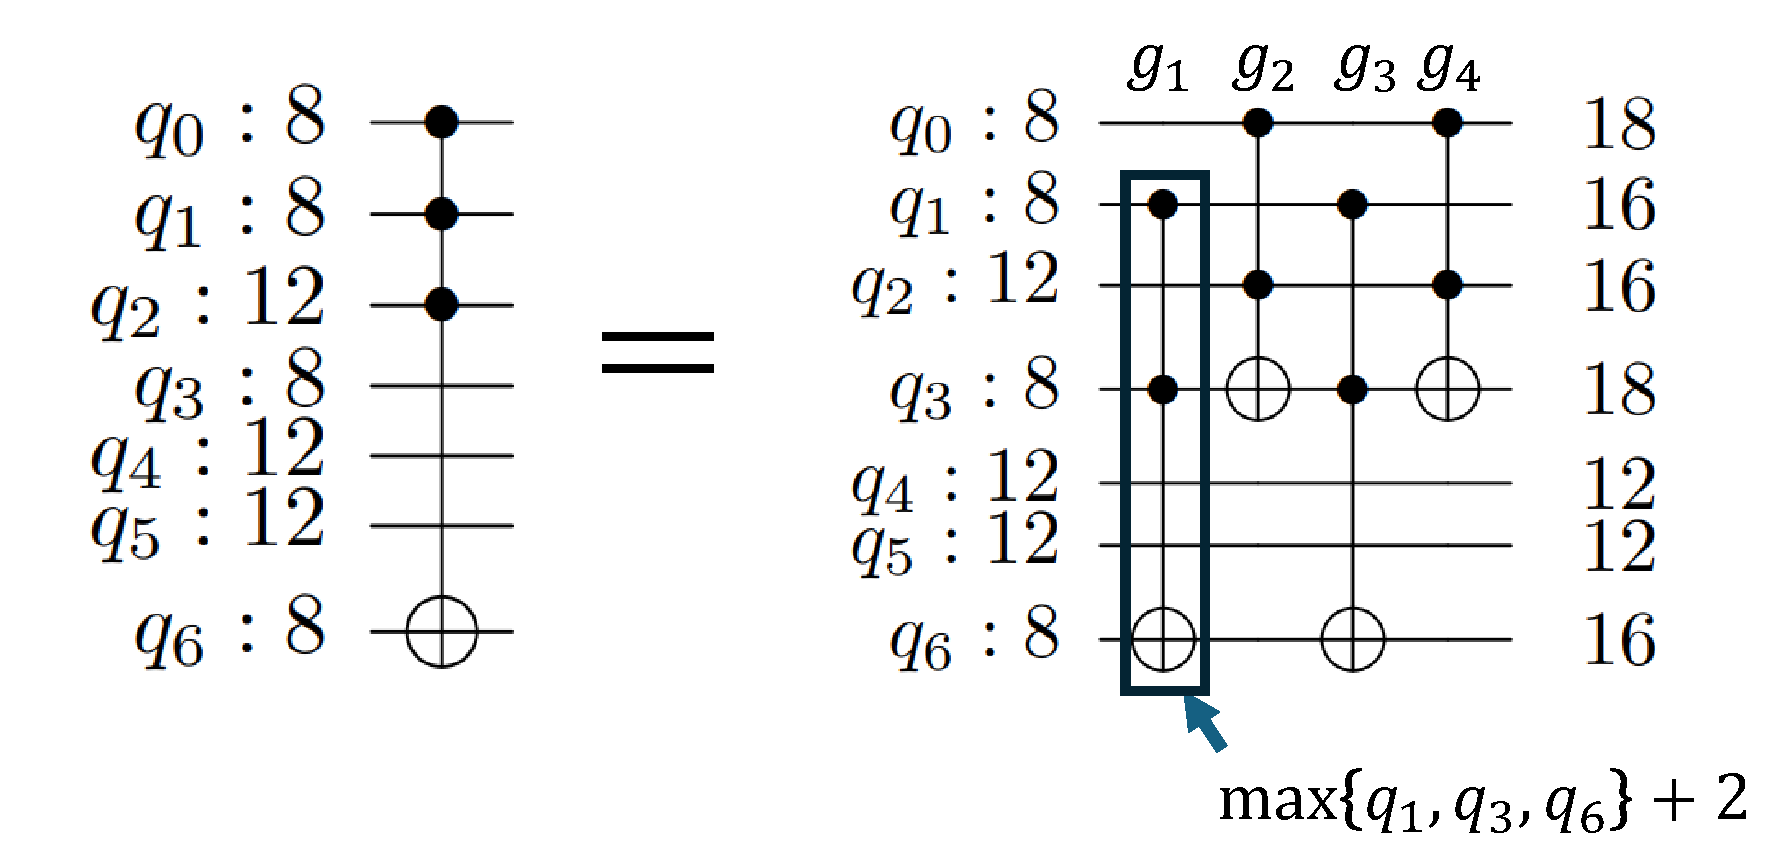
\includegraphics[width=10cm]{img/considering_bit_tdepth.pdf}
\caption{An example of decomposing an MCT gate with 3 control bits while considering the T-depth for each bit}
\label{consider_tdepth}
\end{figure}
\begin{figure}[tbp]
\centering
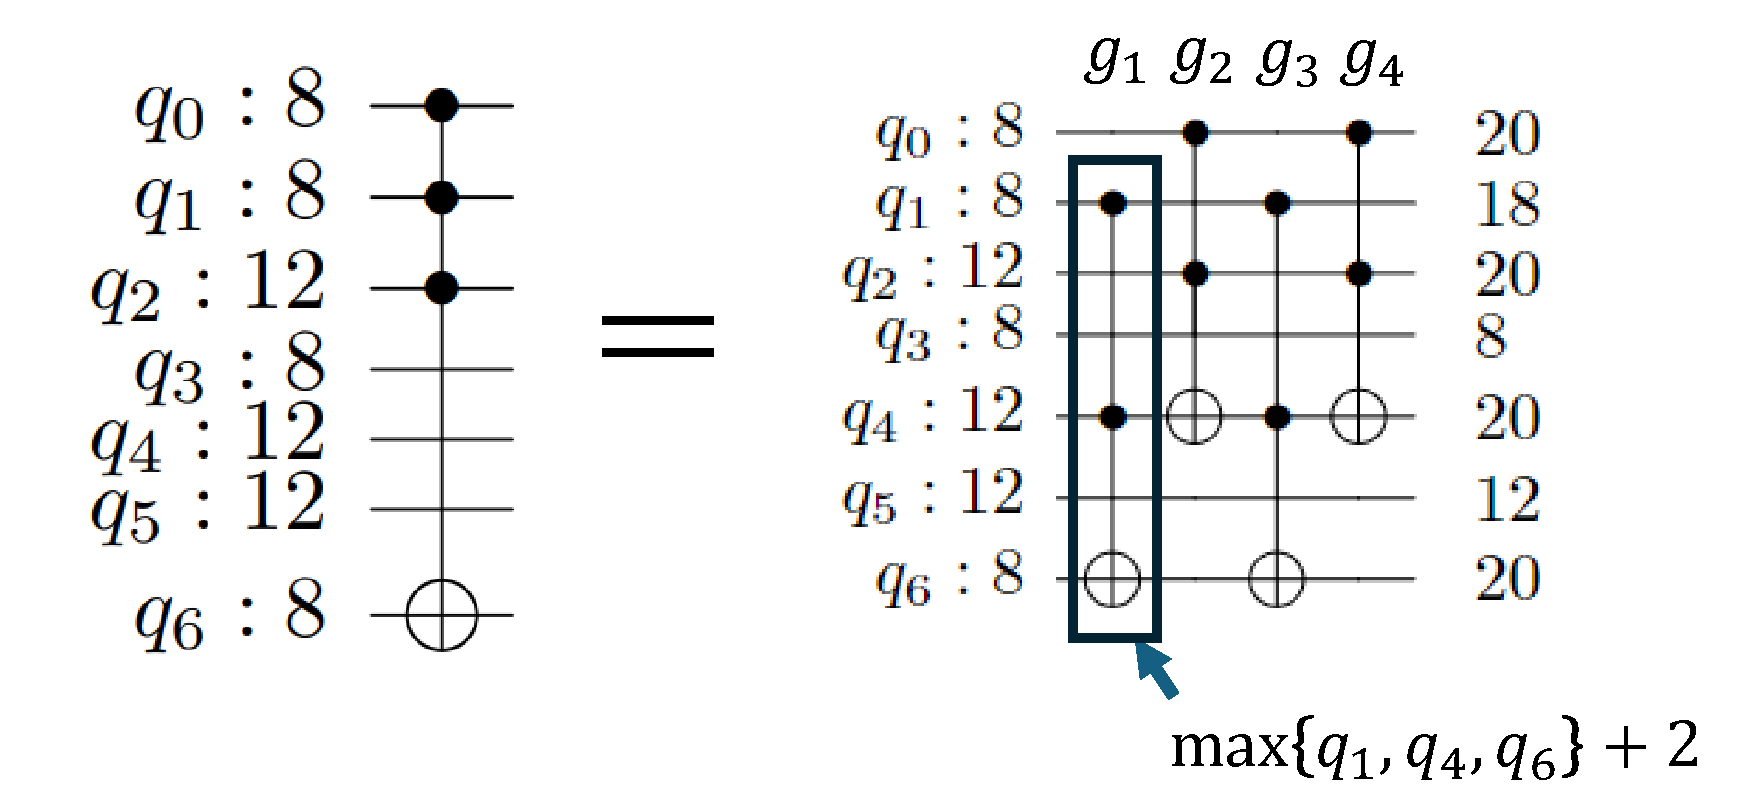
\includegraphics[width=10cm]{img/bad_consider_t-depth.pdf}
\caption{An example of the maximum T-depth deteriorating when decomposing an MCT gate with 3 control bits}
\label{bad_consider_tdepth}
\end{figure}
\subsection{Decomposing MCT gates while considering the T-depth for each bit}
In this section, we explain a method that applies methods 1 to 4 to decomposing MCT gates while considering the T-depth for each bit.
Here, $C$ is the set of $c$ control bits of the MCT gate before decomposition,
and $t$ is the target bit.
\subsection{Method~1}
In this section, we explain how to apply decomposition that considers the T-depth for each bit to Method~1.
\par
Method 1 is a method of decomposing an MCT gate with three or more control bits into a Toffoli gate,
and then replacing the Toffoli gate with a $CCiZ, CCi\omega Z$ gate.
Therefore, when decomposing an MCT gate into a Toffoli gate,
the arrangement of the gates is determined.
\par
We explain how to select bits when decomposing an MCT gate into a Toffoli gate.
Once the arrangement of the bits that make up the three Toffoli gates \rout{$g_{1},g_{2},g_{3}$}
from the left in Figure~\ref{barenco} is determined,
the decomposition of the MCT gate is determined, since the gates to the right are copies of these gates.
That is, in the method of decomposing an MCT gate using $c-2$ auxiliary bits with indefinite values~\cite{barenco1995elementary},
the decomposition can be achieved by determining the arrangement of $c-1$ Toffoli gates.
The method of determining the bits that compose these gates is explained below.
\par
Let $c_{1},\dots,c_{c}$ be the control bits of the MCT gate before decomposition
rearranged in ascending order of T-depth.
Let $t$ be the target bit of the MCT gate before decomposition.
Let $g_{1},\dots,g_{c-1}$ be the $c-1$ Toffoli gates from the left after decomposition.
Let $C_{1},\dots,C_{c-1}$ be the set of control bits of $g_{1},\dots,g_{c-1}$.
Let $a_{1},\dots,a_{c-2}$ be the $c-2$ auxiliary bits with indefinite values rearranged in ascending order of T-depth.
The method for determining the bits that make up $g_{1},\dots,g_{c-1}$ is shown below.
\begin{enumerate}[Step 1]
\item Add $a_{1},\dots,a_{c-2}$ one by one to $C_{1}\dots,C_{c-2}$ in order.
\item Add $c_{1},\dots,c_{c-2}$ to $C_{1},\dots,C_{c-2}$ in order.
\item Add $c_{c-1},c_{c}$ to $C_{c-1}$.
\item Let $t$ be the target bit of $g_{1}$.
\item Let $a_{1}, \dots, and a_{c-2}$ be the target bits of $g_{2}, \dots, and g_{c-2}$, in order.
\end{enumerate}
\par
After determining the bits that make up $g_{1}, \dots, and g_{c-1}$ according to the above procedure,

place the Toffoli gates from the left side of the circuit in the order of equation~\ref{eq:toffoli_haiti}.
\begin{equation}\label{eq:toffoli_haiti}
\{g_{1}, g_{2}, \dots g_{c-1}\},\{g_{c-2},g_{c-3},\dots g_{1}\}, \{g_{2},g_{3},\dots ,g_{c-1}\}, \{g_{c-2}, g_{c-3}\dots ,g_{2}\}
\end{equation}
Finally, these gates are replaced with $CCiZ, CCi\omega Z$ gates using method ~1.
In this way, by placing bits with smaller T-depth in order from the Toffoli gate on the left,
it is possible to prevent bits with larger T-depth from being used first.
\par
Figure ~\ref{b2mapping_proposed} shows an example of decomposing an MCT gate with 4 control bits using method ~1, taking into account the T-depth for each bit.
If the control bits of the MCT gate before decomposition on the left side of Figure~\ref{b2mapping_proposed} are rearranged in order of decreasing T-depth,

$C=\{c_{3}, c_{2}, c_{4}, c_{1}\}$.

The auxiliary bits with indefinite values have decreasing T-depth in the order of $a_{1}, a_{2}$.

First, determine the bits that make up $g_{1}, g_{2}, g_{3}$.

If the control bits of $g_{1}$ are selected in order of decreasing T-depth,

they become $c_{3}, a_{1}$,

and the target bit is $t$.

Next, if the control bits of $g_{2}$ are selected in order of decreasing T-depth,

they become $c_{2}, a_{2}$,

and the target bit is $a_{1}$.

Finally, the control bits of $g_{3}$ are $c_{4}, c_{1}$,
and the target bit is $a_{2}$.
In this way, the bits that make up $g_{1}, g_{2}, and g_{3}$ are determined,
and the Toffoli gates are placed in the order of equation~\ref{eq:toffoli_haiti}.
If the placed Toffoli gates are replaced with $CCiZ, CCi\omega Z$ gates using method~1,
it will look like the right side of Figure~\ref{b2mapping_proposed}. The maximum T-depth in this case is 24.
\begin{figure}
\centering
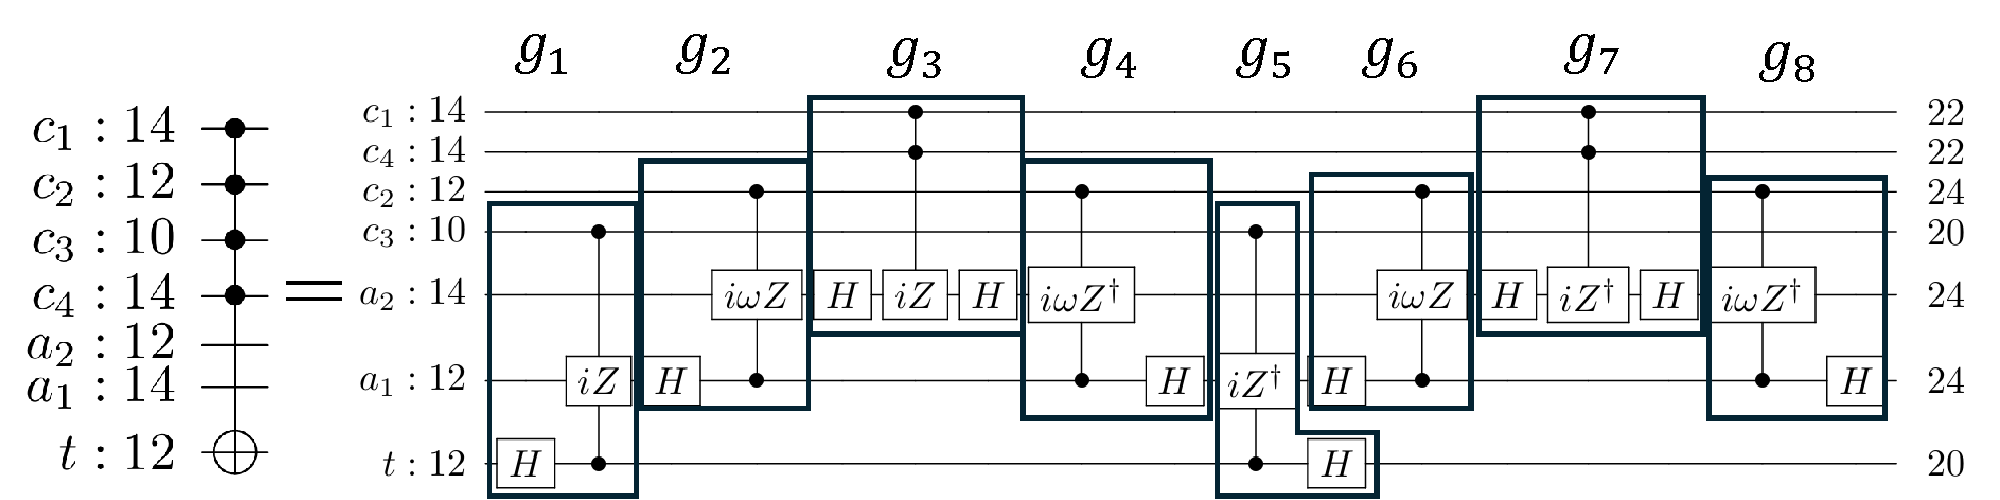
\includegraphics[width=18cm]{img/b2_mapping_proposed.pdf}
\caption{An example of decomposing an MCT gate with 4 control bits using method 1, taking into account the T-depth for each bit}
\label{b2mapping_proposed}
\end{figure}

\begin{comment}
\begin{algorithm}[tbp]
\caption{Decomposition taking into account the T-depth for each bit}\label{alg:b2map_bit}
\begin{algorithmic}[1]
\Require $tdepth\Leftarrow$ T-depth for each quantum bit
\Require $C\Leftarrow$ List of control bits for the MCT gate to be decomposed
\Require $t\Leftarrow$ Target bit for the MCT gate to be decomposed
\Require $D\Leftarrow$ List of uninitialized auxiliary bits
\Ensure $circ$: Decomposed MCT gate
\State $C \Leftarrow$ Sort the list of control bits in ascending order of T-depth
\State $D \Leftarrow$ Sort the list of auxiliary bits in ascending order of T-depth
\For{$(q,index) \leftarrow $C elements and their indexes}
\If{$i==0$}
\State
\EndIf
\EndFor
\end{algorithmic}
\end{algorithm}
\end{comment}
\subsection{Method 2}
In this section, we explain how to apply the decomposition that takes into account the T-depth of each bit to Method 2.
\par
In Method 2, the MCT gate is decomposed into four $C\omega S$ gates and four MCT gates.
First, we explain how to determine the bits that compose the four $C\omega S$ gates and four MCT gates that appear in the decomposition.
Let $a$ be a bit with an indefinite value.
First, the four $C\omega S$ gates have one undefined auxiliary bit $a$ as the control bit,
and $t$ as the target bit.
Next, the four MCT gates that appear in the decomposition are $g_{1},\dots, g_{4}$ from the left.
We will explain how to determine the bits that make up $g_{1} and g_{2}$.
The sets of control bits for $g_{1} and g_{2}$ are $C_{1} and C_{2}$.
The $c$ control bits of the MCT gates before decomposition
sorted in ascending order of T-depth are $c_{1},\dots, c_{c}$.
$C_{1} and C_{2}$ are determined according to the formula~\ref{eq:method2bunkatu}.
\begin{equation}\label{eq:method2bunkatu}
C_{1}=\{c_{1},\dots, c_{\lfloor c/2 \rfloor}\}, C_{2}=\{c_{\lfloor c/2 \rfloor +1},\dots , c_{c}\}
\end{equation}
The target bit of $g_{1} and g_{2}$ is $a$.
As for $g_{3} and g_{4}$, they are copies of $g_{1}$ and $g_{2}$, respectively,
so they are composed of the same bits as these gates.
In this way,
the bits that compose the four $C\omega S$ gates and four MCT gates that appear in the decomposition are determined.
\par
After determining the four $C\omega S$ gates and the bits that make up the four MCT gates that appear in the decomposition,
these gates are decomposed in order from the left, and the T-depth update for each bit is repeated.
These gates are decomposed and placed according to Algorithm~\ref{alg:method2_placement_decomp}.
In this way, by decomposing from the left gate,
each gate can be decomposed while taking into account the T-depth for each bit.
\begin{algorithm}[tbp]
\caption{Decomposition and placement of method 2 considering T-depth for each bit}
\label{alg:method2_placement_decomp}
\begin{algorithmic}[1]
\Require MCT gates $g_{1},\dots, g_{4}$
\Require $C\omega S$ gates
\Require Correspondence between each bit $c_{1},\dots, c_{c}, a, t$ and T-depth
\Ensure Circuit $OC$ consisting of gates that can be decomposed into Clifford+T without using auxiliary bits
\State $C_{i}$ is a set of control bits for $g_{i}$
\For{i={1,\dots ,2}}
\State $C\omega S$ gates are added to $OC$, and the T-depth for each bit is updated
\State $C_{(i+1)\% 2}$, extract $|C_{i}|-2$ bits in ascending order of T-depth.
\State Using the extracted $|C_{i}-2|$ bits as auxiliary bits, decompose $g_{i}$ using method ~1, taking into account the T-depth of each bit.
\State Add the decomposition result of $g_{i}$ to $OC$, and update the T-depth of each bit.
\EndFor
\For{i={1,\dots ,2}}
\State Add a $C\omega S$ gate to $OC$.
\State Add the decomposition of $g_{i}$ to $OC$ by replacing it with an inverse transformation gate and reversing the order.
\EndFor
\end{algorithmic}
\end{algorithm}
\par
\begin{figure}
\centering
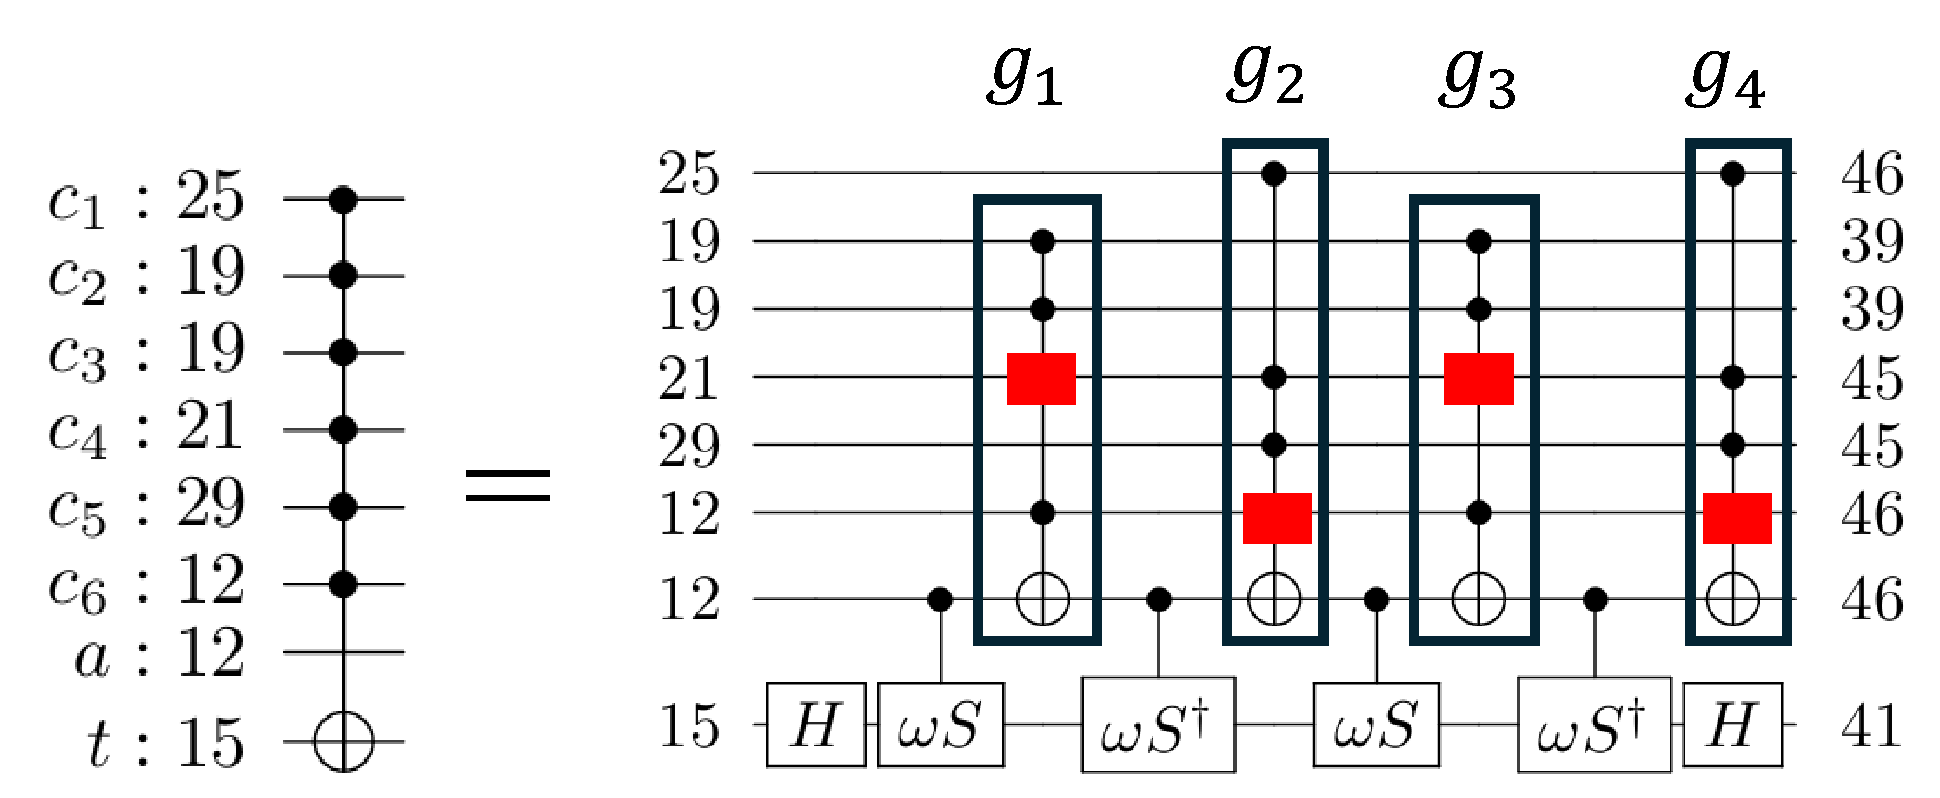
\includegraphics[width=10cm]{img/mimap_proposed.pdf}
\caption{An example of decomposing an MCT gate with 6 control bits using method ~2, taking into account the T-depth for each bit}
\label{mimap_proposed}
\end{figure}
\bout{Figure ~\ref{mimap_proposed} shows an example of decomposing an MCT gate with $c=6$ into four MCT gates and four $C\omega S$ gates using method ~2, taking into account the T-depth for each bit.
First, to decompose an MCT gate using method ~2, taking into account the T-depth for each bit,
divide the control bits into two sets in ascending order of T-depth according to equation ~\ref{eq:method2bunkatu}.
In the example of Figure~\ref{mimap_proposed}, $C_{1}=\{c_{6}, c_{2},c_{3}\}, C_{2}=\{c_{1}, c_{4}, c_{5}\}$.

Once the division of the control bits is determined,
the bits that make up the four MCT gates and the $C\omega S$ gate can be determined.

The right side of Figure~\ref{mimap_proposed} is an example of
the MCT gate with $c=6$ decomposed into four MCT gates and
four $C\omega S$ gates. }
\par
\bout{Finally, the gates in the circuit on the right side of Figure~\ref{mimap_proposed} are decomposed according to Algorithm~\ref{alg:method2_placement_decomp}

First, calculate the T-depth of each bit from the decomposition results of gates up to $g_{1}$,
and decompose $g_{1}$ using $c_{3}$ as an auxiliary bit.
Next, decompose $g_{2}$ using $c_{6}$ as an auxiliary bit from the decomposition results of gates up to $g_{2}$.
Finally, $g_{3}$ and $g_{4}$ are replaced with the inverse transformation of the decomposition of $g_{1}$ and $g_{2}$, respectively, and then arranged in reverse order.
By decomposing each gate in this way,
the maximum T-depth of the decomposition result of Figure~\ref{mimap_proposed} is 46. }
\subsection{Method 3}
We explain how to apply decomposition that takes into account the T-depth for each bit to Method~3.
\par
In method ~3, the number of control bits \rout{of each MCT gate after decomposition is determined according to the number of auxiliary bits $m\geq 2$ whose values are indefinite to be used in the decomposition and the number of control bits $c$ of the MCT gate to be decomposed. }
The number of control bits of each MCT gate $g_{1},\dots, g_{m+1}$ after decomposition obtained by method ~3 is set to $N_{1},\dots, N_{m+1}$.

In method ~3, the control bits are preferentially placed in the $1$th and $m+1$th gates, so the value of $N_{2},\dots, N_{m}$ is 2.

\par
First, to determine the decomposition of method ~3, it is necessary to determine the placement of $g_{1},\dots,g_{m+1}$.

However,However, if the number of control bits in $g_{1}$ is three or more, the T-depth of the bits used in $g_{2},\dots, g_{m+1}$ changes depending on the result of the decomposition of $g_{1}$.

Therefore, $g_{1}$ must be decomposed in advance taking into account the T-depth of each bit,
and then the placement of $g_{2},\dots, g_{m+1}$ must be determined depending on the result.

The set of control bits for $g_{1},\dots,g_{m+1}$ is defined as $C_{1},\dots,C_{m+1}$.

The set of $m$ indefinite bits used for the decomposition is defined as $A$.

The placement of $g_{1},\dots,g_{m+1}$ is determined according to the following procedure.
\begin{enumerate}[Step 1]
\item Determine the arrangement of $g_{1}$ and decompose it. Update the T-depth of each bit from the result of the decomposition.
\begin{enumerate}
\item Move the element with the smallest T-depth from $A$ to $C_{1}$.
\item Move elements from $C$ in ascending order of T-depth so that $|C_{1}|=N_{1}$.
\item Let $t_{1}=t$.
\item Select $|C_{1}|-2$ bits in ascending order of T-depth from among the bits that are not $C_{1}$ or $t$.
\item Using the selected bits as auxiliary bits, decompose $g_{1}$ using method ~1, taking into account the T-depth of each bit.
\item Update the T-depth of each bit from the result of the decomposition.
\end{enumerate}
\item Select and place bits from $g_{2}, \dots ,g_{m+1}$ in ascending order of T-depth.
\begin{enumerate}[(1)]
\item Let $i=2$.
\item Move the element of $A$ with the smallest T-depth to $C_{i}$.
\item Move elements from $C$ in ascending order of T-depth so that $|C_{i}|=N_{i}$.
\item Let $t_{i}$ be the element of $A$ moved to $g_{i-1}$.
\item As long as $i < m+1$, set $i=i+1$ and return to (2). Otherwise, exit.
\end{enumerate}
\end{enumerate}
The placement of $g_{1},\dots, and g_{m+1}$ is determined using this procedure.
After that,
according to Algorithm~\ref{alg:method3_placement_decomp},
we repeat the decomposition and bitwise T-depth updates,
and decompose and place the MCT gates in the order of formula~\ref{eq:bakerhaiti}.
\begin{algorithm}[tbp]
\caption{Placement and decomposition of method 3 considering T-depth for each bit}
\label{alg:method3_placement_decomp}
\begin{algorithmic}[1]
\Require List of MCT gates in formula ~\ref{eq:bakerhaiti}: $mctlist$
\Require Correspondence between each bit and T-depth
\Ensure Circuit composed of gates that can be decomposed into Clifford+T without using auxiliary bits: $OC$
\For{$g \leftarrow mctlist$}
\State Set of unused bits in \State $g$: $A$
\State Number of control bits in \State $g$: $c$
\State Extract $c-2$ bits from \State $A$ in ascending order of T-depth.
\State Using the extracted $c-2$ bits as auxiliary bits, $g$ is decomposed using method~1, taking into account the T-depth for each bit.
\State Add the decomposition result of $g$ to $OC$, and update the T-depth for each bit.
\EndFor
\end{algorithmic}
\end{algorithm}
\par
Figure~\ref{baker_proposed} shows an example of decomposing an MCT gate with $c=5$ using method~3, which takes into account the T-depth for each bit.
We will explain the decomposition of Figure~\ref{baker_proposed}.
First,
using method~3,
the number of control bits for each gate when decomposing the gate on the left side of Figure~\ref{baker_proposed} is calculated,
which is $N_{1}=3, N_{2}=2, N_{3}=2$.
Next, determine the bits that make up $g_{1}, g_{2}, g_{3}$ in order.
First, determine the control bit $C_{1}$ of $g_{1}$.

Of the auxiliary bits $a_{1}, a_{2}$, move the bit $a_{2}$ with the smallest T-depth to $C_{1}$.

Also, select two bits, $c_{2} and c_{5}$, from $c_{1},\dots,c_{5}$ in ascending order of T-depth value and move them to $C_{1}$.

Let $t$ be the target bit of $g_{1}$.

Since the number of control bits of $g_{1}$ is 3, the bits that make up the subsequent gates will change depending on the decomposition result of $g_{1}$.

Therefore, select $|C_{1}|-2$ bits in ascending order of T-depth from the bits not used by $g_{1}$, and decompose $g_{1}$.

In the example in Figure~\ref{baker_proposed}, $c_{3}$ is treated as an auxiliary bit, $g_{1}$ is decomposed, and the T-depth is recalculated.
After recalculation, the T-depth of each bit is $c_{2}=27, c_{3}=27, c_{5}=27, a_{2}=25, t=25$.
From this result, the bits that make up $g_{2} and g_{3}$ are determined.
The control bits of $g_{2}$ are $a_{1}$, and
of $c_{1}, c_{3}, and c_{4}$, $c_{1}$ is the bit with the smallest T-depth.
Additionally, the target bit of $g_{2}$ is $a_{2}$.
The control bits of $g_{3}$ are the remaining control bits $c_{3}, c_{4}$,
and the target bit is $a_{1}$.

In this way, the bits that make up $g_{1}, g_{2}, g_{3}$ are determined,
and the decomposition on the right side of Figure~\ref{baker_proposed} can be realized by arranging them in the order of equation~\ref{eq:bakerhaiti}.
\par
\bout{Finally, the gates $g_{1},\dots, g_{8}$ on the right side of Figure~\ref{baker_proposed}
are decomposed and arranged from the left side according to Algrorithm~\ref{alg:method3_placement_decomp},
and the decomposition of Method~3, which takes into account the T-depth for each bit, can be determined.

First, $g_{1}$ is decomposed using $c_{3}$, which has the smallest T-depth, as an auxiliary bit.

$g_{5}$ is decomposed using the smallest T-depth bit $c_{4}$ from the decomposition results of $g_{1},\dots, g_{4}$ as an auxiliary bit.
After decomposing all gates, the maximum T-depth is 41. }
\begin{figure}[tbp]
\centering
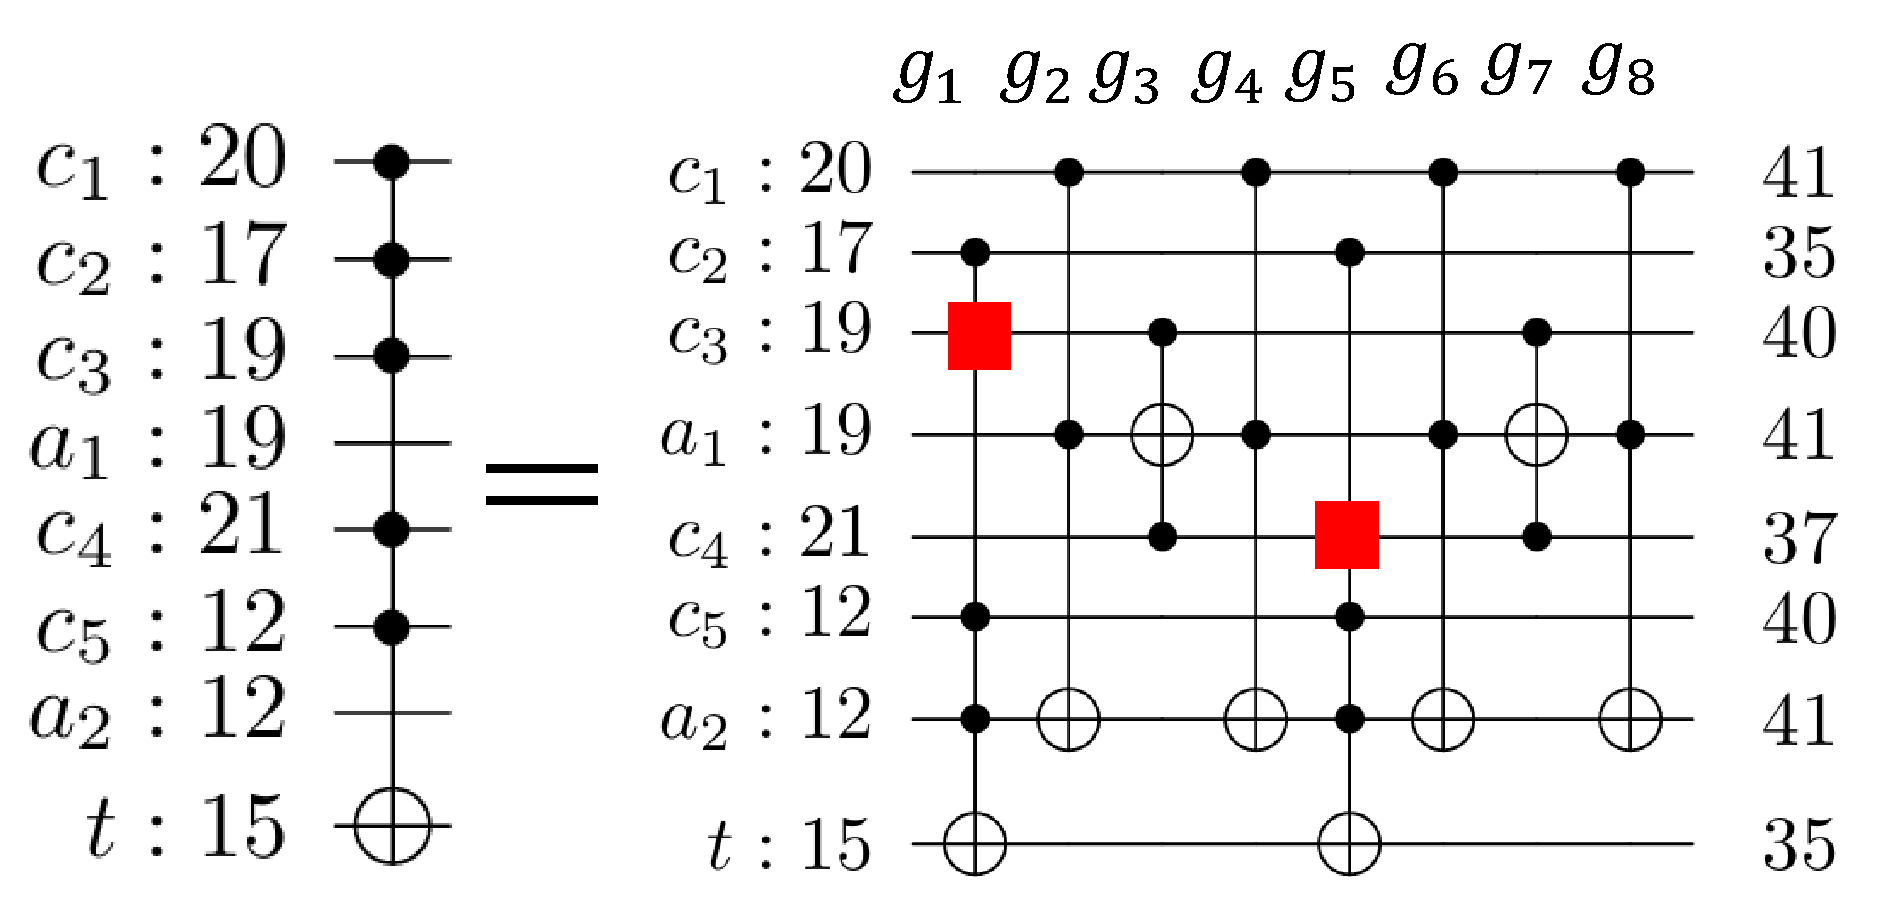
\includegraphics[width=10cm]{img/baker_proposed.pdf}
\caption{An example of decomposing an MCT gate with $c=5$ using method 3, taking into account the T-depth of each bit, with two auxiliary bits of indefinite value}
\label{baker_proposed}
\end{figure}
\begin{comment}
\begin{algorithm}[tbp]
\caption{Placement and decomposition of method 3, taking into account the T-depth of each bit}
\label{alg:method3_placement_decomp}
\begin{algorithmic}[1]
\Require MCT gate before decomposition $(C, t)$ \Comment{$C$ is a set of control bits, $t$ is a target bit}
\Require List of $m$ auxiliary bits $A$
\Require T-depth of each bit
\Ensure $OC$ is a circuit consisting of gates that can be decomposed into Clifford+T without using auxiliary bits.

\State List of empty bits $C_{1},\dots ,C_{m+1}$

\State $m+1$ bits $t_{1},\dots, t_{m+1}$

\State $t_{1} \leftarrow t$

\State $C_{1}$ adds the bit with the smallest T-depth in $A$

\State $t_{2} \leftarrow A$ the bit with the smallest T-depth

\State $A$ removes the bit with the smallest T-depth

\State $C \leftarrow$ Control bits of MCT gate before decomposition

\While{$|C_{1}|-2 \leq c+m-1$ and $|C|\geq m$}

\State $C_{1}$ adds the bit with the smallest T-depth in $C$

\State $C$ removes the bit with the smallest T-depth
\EndWhile
\State $g_{1}\leftarrow (C_{1}, t_{1})$
\State $g_{1}$ is decomposed using $|C_{1}|-2$ bits that are not part of $g_{1}$
\State $g_{1}$ decomposition is added to $OC$
\State $g_{1}$ decomposition is updated for each bit
\For{$i={2,\dots ,m}$}
\State $A$ element with minimum T-depth is added to $C_{i}$
\State $t_{i+1}\leftarrow A$ element with minimum T-depth
\State $A$ element with minimum T-depth is deleted
\State $C$ element with minimum T-depth is added to $C_{i}$
\State $C$ element with minimum T-depth is deleted
\State $g_{i}\leftarrow (C_{i}, t_{i})$
\State Replace $g_{i}$ with $CCi\omega Z$ gate

\State Add $g_{i}$ to $OC$

\EndFor

\State Update the T-depth of each bit

\State $C_{m+1} \leftarrow C$

\If{$|C_{m+1}|=2$}

\State Replace $g_{m+1}$ with $CCiZ$ gate

\State Add $g_{m+1}$ to $OC$

\Else

\State Among the bits that do not constitute $g_{m+1}$, extract $|C_{m+1}|-2$ bits in ascending order of T-depth.

\State Decompose $g_{m+1}$ by using the extracted bits as auxiliary bits, taking into account the T-depth of each bit

\EndIf

\end{algorithmic}
\end{algorithm}
\end{comment}
\subsection{Method 4}
We will explain how to decompose Method 4 by considering the T-depth for each bit.
\par
In Method 4, MCT gates are decomposed into multiple stages according to the number of auxiliary bits used in the decomposition.
The number of control bits for each decomposed MCT gate changes according to the number of auxiliary bits used and the number of control bits for the MCT gate to be decomposed.
The number of auxiliary bits with indefinite values used in the decomposition is $d$, and the number of auxiliary bits with a value of 0 used in the decomposition is $k$.
The number of control bits for the MCT gates in each stage can be calculated from Method 4 using these $c, k, and d$ values.
When MCT gates are decomposed using Method 4, it is assumed that they can be decomposed into $n$ stages. In this case, $n$ is an odd number equal to or greater than 3.
The number of control bits for the MCT gates in each stage is expressed using a two-dimensional array as shown in the formula~\ref{eq:niemann_cnt}.
In equation~\ref{eq:niemann_cnt},
of the gates in the $n$th stage, the MCT gates in the $\lceil \frac{n}{2} \rceil+1$th stage and beyond are omitted because they are copies of the gates in the first stage to the $\lceil \frac{n}{2} \rceil -1$th stage.
The subscript $N$ indicates the stage number and the MCT gate number.
For example, $N_{i, j}$ indicates the number of control bits of the $j$th MCT gate in the $i$th stage.
The $\lceil \frac{n}{2} \rceil$th stage is the central stage, so there is only one gate in this stage.
Therefore, $m_{\lceil \frac{n}{2} \rceil}=1$.
\begin{equation}\label{eq:niemann_cnt}
 \begin{pmatrix}
 N_{1,1} & N_{1,2} & \dots & N_{1,m_{1}} \\
 N_{2,1} & N_{2,2} & \dots & N_{2,m_{2}} \\
 \vdots & \vdots & \ddots & \vdots \\
 N_{\lceil \frac{n}{2} \rceil,1} & N_{\lceil \frac{n}{2} \rceil,2} & \dots & N_{\lceil \frac{n}{2} \rceil,m_{\lceil \frac{n}{2} \rceil}} \end{pmatrix}
\end{equation}
Using this formula~\ref{eq:niemann_cnt}, the number of control bits for each stage of the decomposition in Figure~\ref{niemann_c_2} is shown in
formula~\ref{eq:niemann_c_2}.
\begin{equation}\label{eq:niemann_c_2}
\begin{pmatrix}
2 & 2 & 2 & 2 \\
2 & 2 & & \\
2 & & & \\
2 & & & \\
\end{pmatrix}
\end{equation}
\par
In the proposed method, the placement and decomposition of the MCT gates after decomposition are determined according to the number of control bits for the MCT gates at each stage obtained by method~4.
The set of $k$ auxiliary bits with a value of 0 that can be used for decomposition is called $CA$.
The bits that make up the MCT gate at $\lceil \frac{n}{2} \rceil$ stage are determined by the following procedure.
\begin{enumerate}[Step 1]
\item Let $i=1$.
\item Prepare empty sets $C_{1},\dots ,C_{m_{i}}$. Let $j=1$.
\item Move elements from $C$ in ascending order of T-depth so that $|C_{j}|=N_{i, j}$.
\item If $j<m_{i}$, set $j=j+1$ and return to step 3.
\item Move the bits with the smallest T-depth of $CA$ to $t_{1},\dots, t_{m_{i}}$ one by one in order.
\item Let $C_{1},\dots, C_{m_{i}}$ be the control bits of gate $g_{i, 1},\dots, g_{i, m_{i}}$, and $t_{1},\dots ,t_{m_{i}}$ be the target bits.
\item Find the set $A$ of unused bits in $g_{i, 1},\dots ,g_{i, m_{i}}$.
\item Let $k=1$.
\item To avoid using the same auxiliary bits,
select $|C_{m_{k}}-2|$ auxiliary bits from $A$ in ascending order of T-depth, and delete those elements from $A$.
\item Using the selected auxiliary bits,
decompose $g_{i, k}$ using method 1,
taking into account the T-depth for each bit.
\item If $k < m_{i}$, set $k=k+1$ and return to step 9. Otherwise, proceed to the next step.
\item Update the T-depth of each bit.
\item Add $t_{1},\dots, t_{m_{i}}$ to $C$.
\item If $i< \lceil \frac{n}{2} \rceil$, set $i=i+1$ and return to step 2.
\item Let $C$ be the control bit of the MCT gate $g_{\lceil \frac{n}{2} \rceil, 1}$, and $t$ be the target bit.
\end{enumerate}
The above steps determine the bits that make up the MCT gate at the $1,\dots ,\lceil \frac{n}{2} \rceil$ stage.
The MCT gates at each stage that determine the constituent bits have information, including duplication, in the form of equation~\ref{eq:niemann_gates}.
\begin{equation}\label{eq:niemann_gates}
 \begin{pmatrix}
 g_{1,1} & g_{1,2} & \dots & g_{1,m_{1}} \\
 g_{2,1} & g_{2,2} & \dots & g_{2,m_{2}} \\
 \vdots & \vdots & \ddots & \vdots \\
 g_{\lceil \frac{n}{2} \rceil,1} & g_{\lceil \frac{n}{2} \rceil,2} & \dots & g_{\lceil \frac{n}{2} \rceil,m_{\lceil \frac{n}{2} \rceil}}\\
 g_{\lceil \frac{n}{2} \rceil -1, 1} & g_{\lceil \frac{n}{2} \rceil-1 ,2}& \dots & g_{\lceil \frac{n}{2} \rceil-1 ,m_{\lceil \frac{n}{2} \rceil-1}}\\
\vdots & \vdots & \ddots &\vdots \\
g_{1,1} & g_{1,2} & \dots & g_{1,m_{1}} \\
\end{pmatrix}
\end{equation}
\par
The decomposition of method 4 can be determined by decomposing the MCT gates in
formula~\ref{eq:niemann_gates},
which determine the constituent bits, using method 1,
taking into account the T-depth for each bit.
According to Algorithm~\ref{alg:method4_placement_decomp},
we repeatedly decompose and place the MCT gates in
the formula~\ref{eq:niemann_gates} to determine the decomposition.
\begin{algorithm}[tbp]
\caption{Decomposition and placement of method 4 considering T-depth for each bit}
\label{alg:method4_placement_decomp}
\begin{algorithmic}[1]
\Require 2D array of MCT gates in formula ~\ref{eq:niemann_gates}: $mctlist$
\Require Correspondence between each bit and T-depth
\Ensure Circuit composed of gates that can be decomposed into Clifford+T without using auxiliary bits: $OC$
\For{$pqgate \leftarrow mctlist$}
\State Set of bits not used in $pqgate$: $A$
\For{$g\leftarrow pqgate$}
\State Number of control bits in $g$: $c$
\State Extract $c-2$ bits from \State $A$ in ascending order of T-depth.
\State Delete the extracted $c-2$ bits from \State $A$.
\State Using the extracted $c-2$ bits as auxiliary bits, $g$ is decomposed using method ~1, taking into account the T-depth for each bit.

\State Add the decomposition result of $g$ to $OC$.

\EndFor

\State Update the T-depth for each bit.

\EndFor

\end{algorithmic}
\end{algorithm}
\par
\begin{figure}

\centering

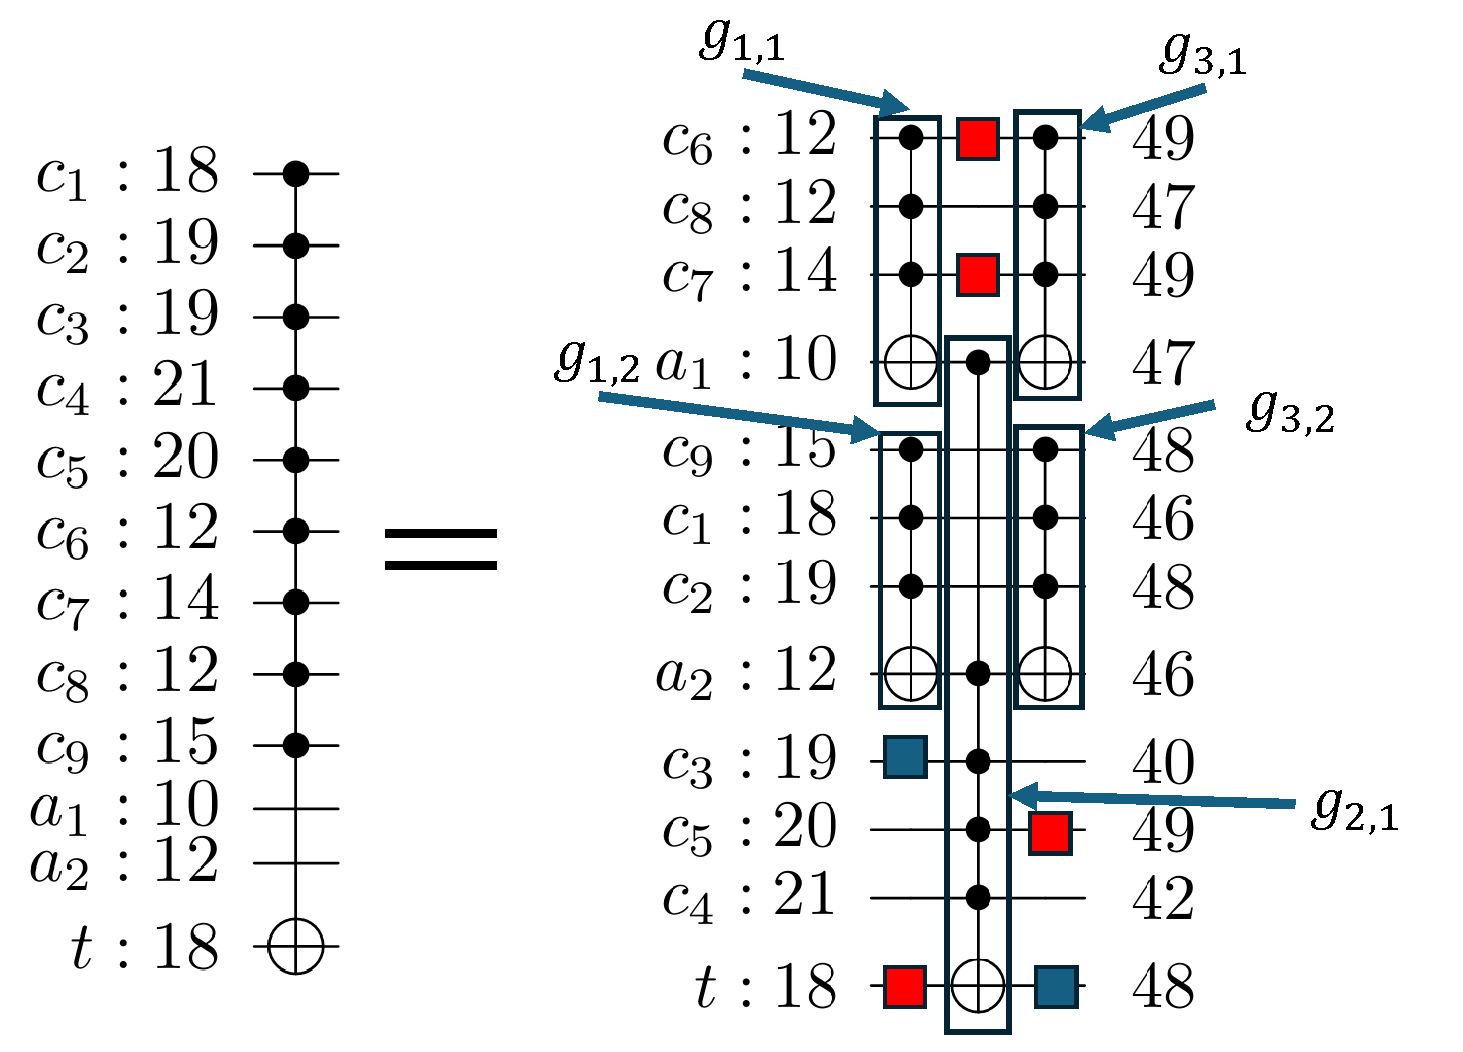
\includegraphics[width=10cm]{img/niemann_proposed.pdf}

\caption{An example of decomposing an MCT gate with $c=9$ using two auxiliary bits with a value of 0,
taking into account the T-depth for each bit, and method~4.}

\label{niemann_proposed}

\end{figure}

Figure ~\ref{niemann_proposed} shows an example of decomposing an MCT gate with $c=9$ using two auxiliary bits with a value of 0,
taking into account the T-depth for each bit, and method~4.
In Figure~\ref{niemann_proposed},
the control bits of the MCT gate before decomposition are $C=\{c_{1},\dots, c_{9}\}$, and the target bit is $t$.

The auxiliary bits with a value of 0 are $CA=\{a_{1}, a_{2}\}$.

First, the number of control bits of the MCT gate at each stage is calculated using method~4, as shown in equation~\ref{eq:niemann_ctrl_gutairei}.

\begin{equation}\label{eq:niemann_ctrl_gutairei}
\begin{pmatrix}

3 & 3 \\

5 & \\
\end{pmatrix}
\end{equation}
The bits that make up each gate are determined according to the number of control bits in equation~\ref{eq:niemann_ctrl_gutairei}.

First, determine the bits that make up the gates $g_{1,1} and g_{1,2}$ in the first to second stages.

When the control bits are selected from $C$ in ascending order of T-depth,
the control bits of the gates in the first stage are $C_{1,1}=\{c_{6}, c_{8}, c_{7}\}$ and $C_{1,2}=\{c_{9}, c_{1}, c_{2}\}$, respectively.

The selected control bits are $C$Then, the target bits for the first-stage gate are selected in ascending order of T-depth, which are $a_{1}$ and $a_{2}$.
The selected auxiliary bit with a value of 0 is added to $C$ and deleted from $CA$.
After determining the bits that make up the first-stage gates $g_{1,1} and g_{1,2}$,
a set $A$ of bits not used in $g_{1,1} and g_{1,2}$ is obtained.
At this time, $A=\{c_{3}, c_{5}, c_{4}, t\}$.
Of these bits, $c_{3} and c_{5}$ are used as auxiliary bits in ascending order of T-depth, $g_{1,1} and g_{1,2}$ are decomposed, and the T-depth is updated.
Next, the bits that make up the second-stage gate $g_{2,1}$ are determined.
Since the gates in the second stage are the central gates,
the control bits are the remaining $C=\{a_{1},a_{2}, c_{3},c_{5},c_{4}\}$,
and the target bit is $t$.
In this way, the bits that make up $g_{1,1}, g_{1,2}, and g_{2,1}$ are determined.
After determining the bits that make up these gates,
the MCT gates are placed in the order of equation~\ref{eq:niemann_gates},
which results in the decomposition of the right side of Figure~\ref{niemann_proposed}.
\par
\bout{Finally, the gates on the right side of Figure~\ref{niemann_proposed} are decomposed
according to Algorithm~\ref{alg:method4_placement_decomp}.
First, decompose the gates $g_{1,1} and g_{1,2}$ in the first stage.
$g_{1,1}$ is decomposed using the bit $t$ filled in red as the auxiliary bit.

$g_{1,2}$ is decomposed using the bit $c_{3}$ filled in blue as the auxiliary bit.

Next, from the result of the decomposition of $g_{1,1} and g_{1,2}$,
$g_{2,1}$ is decomposed using the bits $c_{6} and c_{7}$ filled in red as the auxiliary bits.

Finally, from the result of the decomposition of $g_{2,1}$,
$g_{3,1} and g_{3,2}$ are decomposed using $c_{5} and t$ as the auxiliary bits, respectively.

When all gates are decomposed in this way, the maximum T-depth is 49. }
% Write on the diagram which auxiliary bits were selected.

\begin{comment}
In the proposed method,
the placement and decomposition of the MCT gates after decomposition are determined according to the number of control bits of the MCT gates in each stage obtained by method 4.
Algorithm~\ref{} shows how to determine the placement and decomposition of the MCT gates in each stage.
\begin{algorithm}[tbp]
\caption{Placement and decomposition of method 3 considering T-depth for each bit}
\label{alg:method3_placement_decomp}
\begin{algorithmic}[1]
\Require MCT gate before decomposition $g=(C,t)$
\Require 2D array $CntList$ showing the number of control bits of MCT gates in each stage obtained by method 4
\Require List of bits with value 0 $CA$
\Require List of bits with indefinite value $DA$
\Require T-depth of each bit
\Ensure circuit after decomposition $OC$
\ForEach{$v$ in $CntList$}
\State $n$: Number of elements of $v$
\State $g_{1},\dots, g_{n}$: MCT gate to be placed
\State $C_{1},\dots ,C_{n}$: Set of control bits of each MCT gate
\State $t_{1},\dots ,t_{n}$: Target bits for each MCT gate
\ForEach{$c$ in $v$ with index $i$}
\For{$j=1$ to $c$}
\State $C_{i}$: Add the bit with the smallest T-depth of $C$
\State $C$: Delete the bit with the smallest T-depth
\EndFor
\State $t_{i}$: Add the bit with the smallest T-depth of $CA$
\State $CA$: Delete the bit with the smallest T-depth
\EndFor
\State $g_{1},\dots ,g_{n}$: Decompose the bits considering the T-depth of each bit so that the same auxiliary bits are not used
\State $OC$: Add decomposition of $g_{1},\dots g_{n}$
\State $OC$: Recalculate T-depth
\State $t_{1},\dots, t_{n}$: Add $C$
\EndFor
\end{algorithmic}
\end{algorithm}
\end{comment}
\subsection{Decomposition in reverse order}
In this section, we explain the decomposition of MCT gates in reverse order.

\begin{figure}[tbp]

\centering

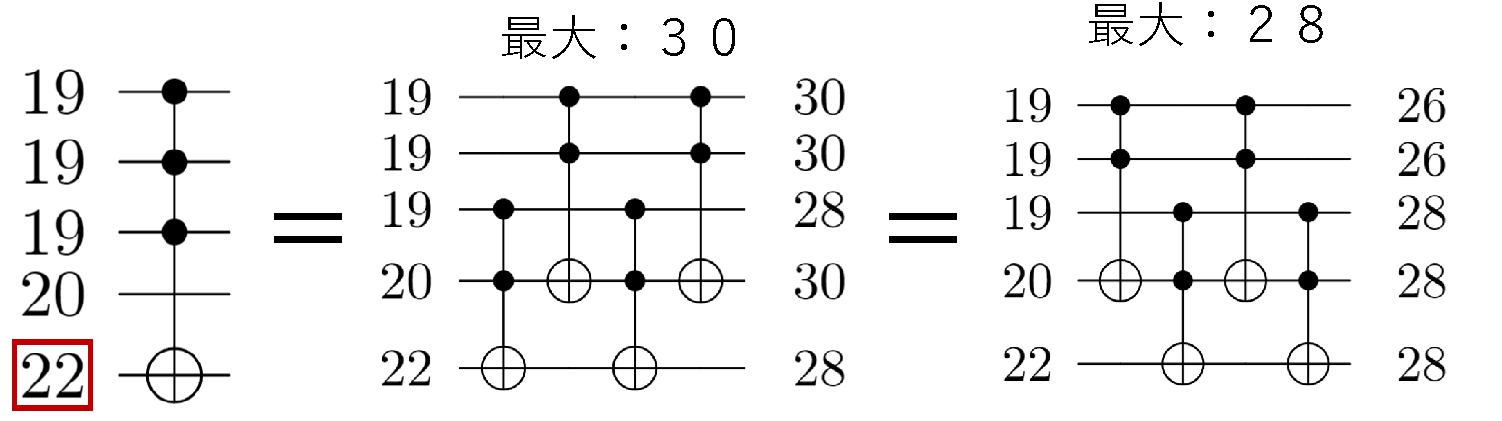
\includegraphics[width=10cm]{img/reverse_mct.pdf}

\caption{Decomposition of an MCT gate with 3 control bits and its decomposition in reverse order}

\label{reverse}

\end{figure}

\par
As shown in Figure~\ref{reverse},
if the T-depth of the target bit is the largest among the auxiliary bits used for the decomposition and the bits that make up the MCT gate to be decomposed,
the T-depth can be reduced by decomposing the MCT gate in reverse order.

The decomposition in the center of Figure~\ref{reverse}
shows the case where the MCT gate on the left side is decomposed in the order of method 1.

On the other hand, the decomposition on the right side shows the case where the MCT gate on the left side is decomposed in the reverse order to the decomposition of method 1.

In the decomposition of the central example, the target bit is always used in the leftmost MCT gate, so the T-depth cannot be reduced.

For this reason, if the T-depth of the target bit is the largest, the T-depth can be reduced by decomposing in reverse order.

In the example in Figure~\ref{reverse}, the maximum T-depth is reduced by 2 by decomposing the MCT gate in reverse order.

\par
To decompose the MCT gate in reverse order using method 1, it is necessary to arrange them in the reverse order of equation~\ref{eq:toffoli_haiti}.

Therefore, it is necessary to use the bits with the smallest T-depth in the order of $g_{2},\dots,g_{c-1},g_{1}$.

The $c$ control bits of the MCT gate before decomposition are rearranged in order of smallest T-depth to be $c_{1},\dots,c_{c}$.
Let $C_{1},\dots,C_{c-1}$ be the set of control bits for $g_{1},\dots,g_{c-1}$.

Let $a_{1},\dots,a_{c-2}$ be the set of $c-2$ undefined auxiliary bits rearranged in ascending order of T-depth.

The method for determining the bits that make up $g_{1},\dots,g_{c-1}$ is shown below.

\begin{enumerate}[Step 1]

\item Let $a_{1}$ be the target bit for $g_{2}$.

\item Add $a_{2},\dots,a_{c-2},a_{1}$ to $C_{2}\dots,C_{c-2},C_{1}$ one by one in order.

\item Add $c_{1}, \dots , and c_{c-3}$ to $C_{2}, \dots , and C_{c-2}$, in that order.
\item Add $c_{c-2} and c_{c-1}$ to $C_{c-1}$.
\item Add $c_{c}$ and $a_{1}$ to $C_{1}$.
\item Let the target bits of $g_{3}, \dots , and g_{c-2}$ be $a_{2}, \dots , and a_{c-3}$, respectively, in that order.
\item Let the target bit of $g_{1}$ be $t$.
\end{enumerate}
After determining the bits that make up $g_{1},\dots, g_{c-1}$,
by arranging them in the reverse order of equation~\ref{eq:toffoli_haiti},
the decomposition of method 1 can be performed in the reverse order.
\par
For method~2, by decomposing in the reverse order, the target bit can be used\bout{later}.
By arranging the four MCT gates $g_{1},\dots, g_{4}$ and the four $C\omega S$ gates in the reverse order, the decomposition in the reverse order can be performed.
The bit with an indefinite value used in the decomposition is $a$.
Even when the four $C\omega S$ gates are decomposed in the reverse order, $a$ remains the control bit and $t$ remains the target bit.
When decomposing in the reverse order, MCT gates are placed from the left in the order of $g_{4}, \dots, g_{1}$, so it is necessary to place bits with small T-depth in $g_{4}, g_{2}$.

Therefore, $C_{2}, C_{1}$ are the sets of control bits for $g_{1}, g_{2}$,
and $C_{1}, C_{2}$ are determined according to equation~\ref{eq:method2bunkatu}.

Once the bits that make up each gate are determined,

by repeating the decomposition and placement in the order of $g_{4}, C\omega S, g_{3}, C\omega S, \dots , g_{1}, C\omega S$,
the decomposition in the reverse order of method~2 can be achieved.

\par
To decompose method 3 in the reverse order,
it is necessary to place the MCT gates decomposed in the reverse order of equation~\ref{eq:bakerhaiti}.
Therefore, it is necessary to arrange the bits with the smallest T-depth in the order of $g_{2}, \dots, g_{m+1}, g_{1}$.

Let $A$ be the set of $m$ auxiliary bits used for decomposition.

Let $N_{1}, \dots, N_{m+1}$ be the number of control bits for each MCT gate $g_{1}, \dots, g_{m+1}$ after decomposition,

obtained by method 3.

Let $C_{1}, \dots, C_{m+1}$ be the set of control bits for $g_{1}, \dots, g_{m+1}$.

Let $t_{1}, \dots, t_{m+1}$ be the target bits for $g_{1}, \dots, g_{m+1}$.

The bits that make up $g_{1},\dots, and g_{m+1}$ are determined according to the following procedure.
\begin{enumerate}[Step 1]
\item Determine the bits that make up $g_{2}$.
\begin{enumerate}
\item Move the element with the smallest T-depth from $A$ to $C_{2}$.
\item Move the element with the smallest T-depth from $A$ to $t_{2}$.
\item Move the element with the smallest T-depth from $C$ to $g_{2}$.
\end{enumerate}
\item Determine the bits that make up $g_{3},\dots, and g_{m+1}$.
\begin{enumerate}
\item Let $i=3$.
\item Move the element with the smallest T-depth from $A$ to $C_{i}$.
\item From $C$ to $N_{i}$ so that $|C_{i}|=N_{i}$.Move elements in ascending order of T-depth.
\item Let $t_{i}$ be the element of $A$ moved to $C_{i-1}$.
\end{enumerate}
\item Determine the bits that make up $g_{1}$.
\begin{enumerate}
\item Add $t_{2}$ to $C_{1}$.
\item Move the remaining elements of $C$ to $C_{1}$.
\item Let $t_{1}$ be $t$.
\end{enumerate}
\end{enumerate}
By using this procedure to determine the bits that make up $g_{1},\dots, and g_{m+1}$, and then arranging the gates in the reverse order of equation~\ref{eq:bakerhaiti},
and decomposing, method 3 can also be decomposed in the reverse order.

As for method 4, since the decomposition is symmetric, there is no change in the T-depth even if the decomposition is performed in the reverse order.
% Methods 2 and 3 are explained separately.
\subsection{Decomposition method using beam search considering subsequent gates}
This section explains the method of decomposing MCT gates using beam search, taking into account subsequent gates.

Figure~\ref{select_ancilla_tdepth} shows the change in T-depth due to the selection of auxiliary bits for two MCT gates $g_{1} and g_{2}$.
The example in the center of Figure~\ref{select_ancilla_tdepth} shows an example in which $g_{1}$ selects the auxiliary bit with the smallest T-depth, which is filled in red, for decomposition, and $g_{2}$ selects the bit with the smallest T-depth, which is filled in blue, based on the result of the decomposition of $g_{1}$.
In the example on the right side of Figure~\ref{select_ancilla_tdepth},
$g_{1}$ selects the auxiliary bit with a T-depth of 41 (filled in red) and decomposes it,
while $g_{2}$ receives the result of the decomposition of $g_{1}$ and selects the bit with the smallest T-depth (filled in blue).
In the example in the center of Figure~\ref{select_ancilla_tdepth},
the maximum T-depth is 58,
while in the example on the right side,
the maximum T-depth is 53.
\begin{figure}[tbp]
\centering
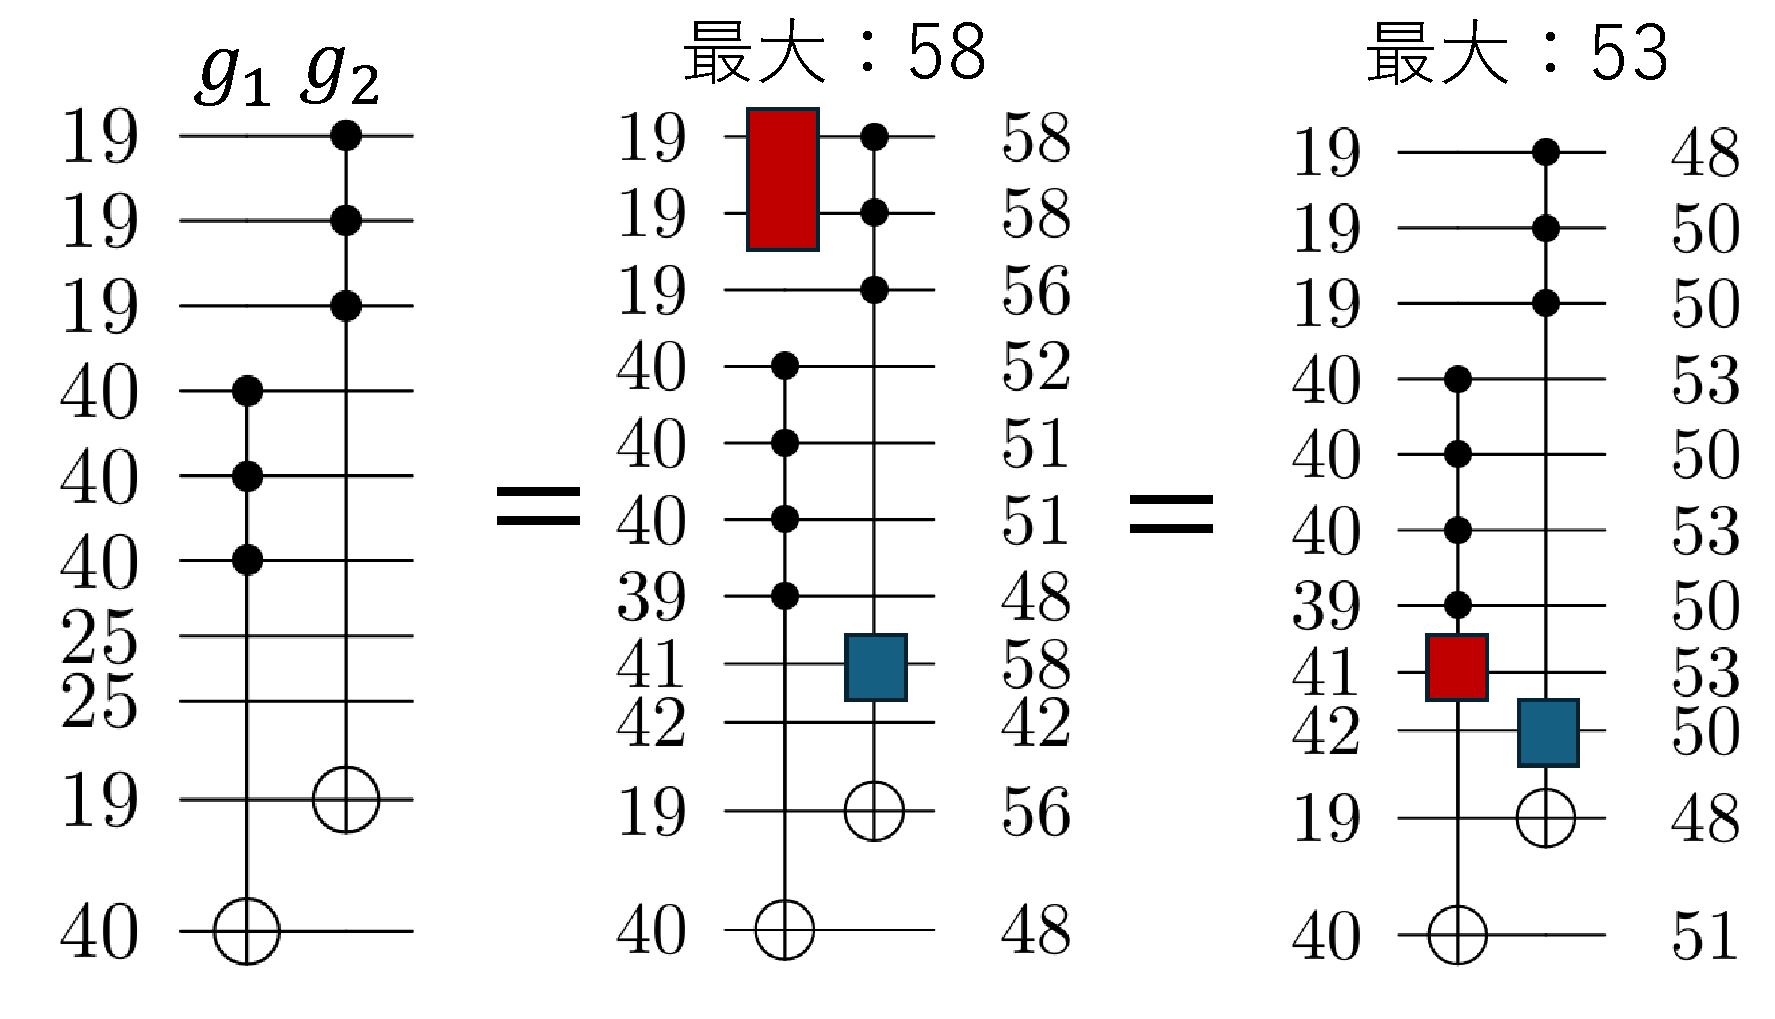
\includegraphics[width=10cm]{img/select_ancilla_biit_tdepth.pdf}
\caption{Example of change in T-depth by selecting auxiliary bits for two MCT gates}
\label{select_ancilla_tdepth}
\end{figure}
As in the central example of Figure~\ref{bad_consider_tdepth},
if a bit with a small T-depth is selected greedily,
the T-depth may worsen when decomposing the \bout{successor} gate.
For this reason, it is necessary to decompose the MCT gate considering the \bout{successor} gate of the gate to be decomposed.
\par
When decomposing MCT gates considering the T-depth for each bit,
the T-depth of each bit changes depending on the result of the decomposition of the MCT gate.
Therefore, a tree is constructed by setting the evaluation value of each node as the maximum T-depth,
and treating the decomposition of each MCT gate as a transition.
The optimal decomposition can be found by exhaustively searching this tree.
However, if a full search is performed, the computational complexity will be enormous as the number of quantum bits and the number of MCT gates to be decomposed increase.

For this reason, we use beam search \cite{bisiani1992beam} to limit the search range to a predetermined number of candidates,
and perform the search while keeping the computational complexity to a realistic level.

Here, we also limit the enumeration of the decompositions of each MCT gate.

To enumerate all the decompositions, we must enumerate all the combinations of the selection of the auxiliary bits.

An MCT gate with $c$ control bits can select $1$ to $c-2$ auxiliary bits with undefined values.

If the number of usable auxiliary bits with undefined values is $m$,
there are $\sum_{i = 1}^{c-2} {}_mC_{i}$ ways to select the auxiliary bits with undefined values.

When the number of quantum bits in the circuit and the number of control bits in the MCT gates that make up the circuit increase,
it is difficult to enumerate all the selections of the auxiliary bits,
so we limit the number of transitions by using the specified decomposition as the transition.
The specified decomposition is as follows.
\begin{enumerate}[(1)]
\item Select 1 to $c-2$ auxiliary bits with undefined values in ascending order of T-depth
\item Select 1 to $c-2$ auxiliary bits with 0 values in ascending order of T-depth
\item Select 1 to $c-2$ bits with undefined values from the bits not used by the gate immediately following the gate performing the decomposition in ascending order of T-depth.
\item Decomposition in reverse order of these decompositions
\end{enumerate}
\par
The pseudo code for beam search is shown in Algorithm~\ref{alg:mct_beam}, where the decomposition of MCT gates is the transition and the maximum T-depth after the decomposition is the evaluation value.
Figure~\ref{mct_beam} shows how the decomposition of $g_{1}$ in Figure~\ref{select_ancilla_tdepth} is determined according to Algorithm~\ref{alg:mct_beam}.

The search width in Figure~\ref{mct_beam} is 3, and the search depth is 2.

For simplicity, the decomposition in reverse order is not enumerated.

First, in Figure~\ref{mct_beam},

the decomposition of $g_{1}$ is enumerated \rout{$D_{1},\dots, D_{4}$. }

The maximum T-depth of the circuit obtained from the decomposition $D_{1},\dots,D_{4}$ is set as the evaluation value of the node.

The nodes are sorted in ascending order of evaluation value,

and the decomposition of the next gate $g_{2}$ is enumerated from the top three nodes.

T-depth is calculated from the result of the decomposition of $g_{2}$,
and the first transition of the node with the smallest evaluation value is determined as the decomposition of $g_{1}$.

In this example, $D_{3}$ is determined as the decomposition of $g_{1}$.

\begin{figure}[tbp]

\centering

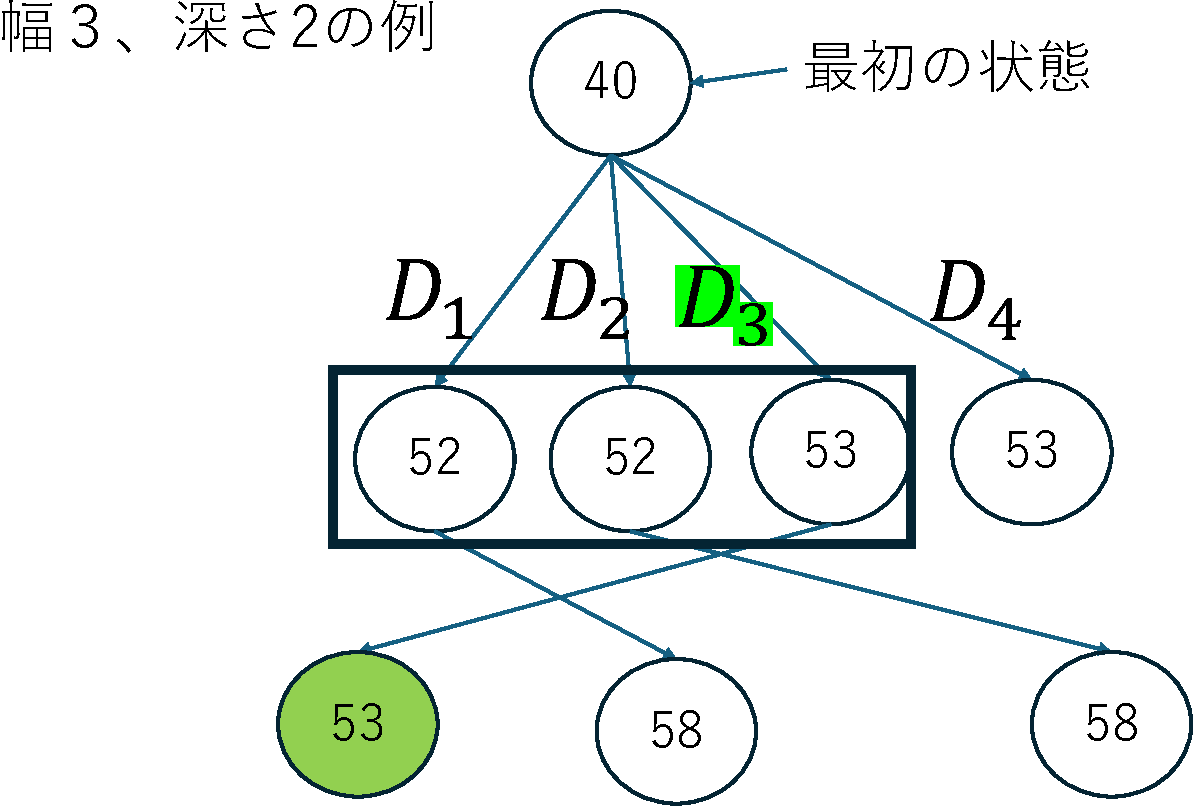
\includegraphics[width=8cm]{img/mct_beam.pdf}

\caption{Figure~\ref{select_ancilla_tdepth} shows how the decomposition of $g_{1}$ is determined according to Algorithm~\ref{alg:mct_beam}}

\label{mct_beam}

\end{figure}

In the proposed method, for a circuit composed of MCT gates, the decomposition is determined gate by gate
based on Algrorithm~\ref{alg:mct_beam}, and all gates are decomposed.

% Should I give a concrete example? The example in the figure is not very good.

\begin{comment}
Figure~\ref{mct_beam} shows how a beam search with a search depth of 2 and width of 3 is used,

Figure~\ref{bad_consider_tdepth} shows how the decomposition of the MCT gate is determined taking into account subsequent gates.
\begin{figure}[tbp]
\centering
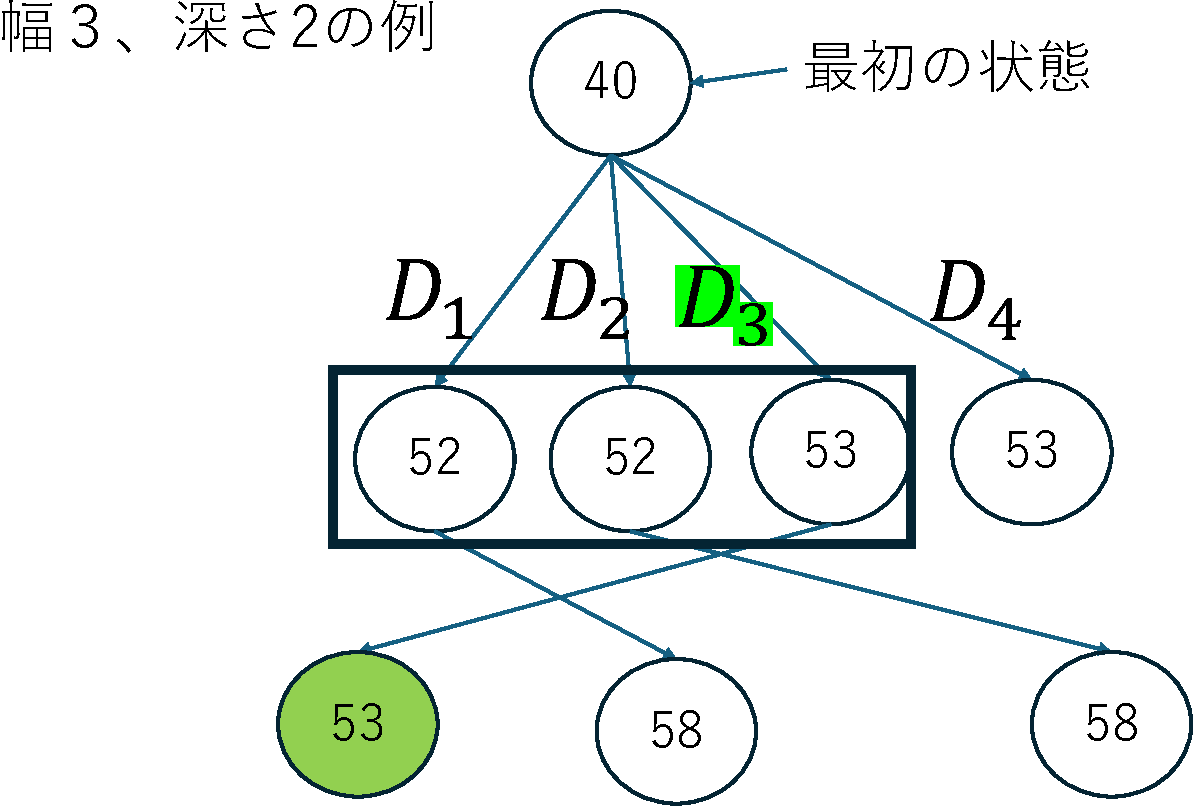
\includegraphics[width=10cm]{img/mct_beam.pdf}
\caption{Example of change in T-depth by selecting auxiliary bits for two MCT gates}
\label{mct_beam}
\end{figure}
\end{comment}

\begin{algorithm}[tbp]
\caption{Pseudocode for beam search with maximum T-depth as evaluation value}
\label{alg:mct_beam}
\begin{algorithmic}[1]
\Require $state$: (maximum T-depth, T-depth per bit, MCT gate to be decomposed)
\Require $legal\_actions$: Function to enumerate decompositions of MCT gates and return the state before the next gate decomposition
\Require $depth$: Depth to search
\Require $width$: Width to search
\State $best\_decomp$: Best candidate
\State $candidate\_list$ List of search candidates, prioritized queue
\State $candidate\_list.push(state)$
\For{$1,..,depth$}
\State $next\_candidate\_list$ List of next search candidates, prioritized queue
\For{$1,..,width$}
\If{If $candidate\_list$ is empty}
\State break
\EndIf
\State $now\_state \Leftarrow candidate\_list.pop()$ Extract the best value of the search candidate and pop it
\State $next\_candidate\_list.push(legal\_actions(now\_state))$ Add the transition from the current state to the list of next search candidates
\EndFor
\State $candidate\_list \Leftarrow next\_candidate\_list$ Update the list of search candidates
\State $best\_decomp \Leftarrow candidate\_list.top()$ Update the best candidate
\EndFor
\State \Return Return the first transition of $best\_decomp$
\end{algorithmic}
\end{algorithm}

%% \input{Exp.tex}
%% \input{Concl.tex}

%\renewcommand{\baselinestretch}{1.2}
\vspace{-0.3cm}
%\renewcommand{\baselinestretch}{1.0}
\bibliographystyle{plain}
\bibliography{ref}
%\vspace{12pt}
\end{document}
